\chapter{Reutilizarea şi modularizarea codului}
\vskip -25pt
\textit{Acest capitol îţi va prezenta tehnici de reutilizare a codului,
ceea ce-ţi va permite să programezi mai eficient. Îţi va
mai deschide porţile şi către mai toate funcţionalităţile
şi capacităţile limbajului PHP.}
\vskip 5em

\section{Funcţii}
\subsection{Funcţii proprii. Termeni generali}
%retval, args, optional args, references, static variables
O funcţie este ca o cutie neagră. O hrăneşti cu date prin
intermediul a ceea ce numim \textsl{parametri}, şi ea
face anumite operaţii pe acel input primit prin parametri.

Unele funcţii generează output, alte funcţii returnează
valori şi nu afişează nimic, iar altele nici nu acceptă
parametri.

Până acum am întâlnit o singură funcţie, \texttt{var\_dump()}.
Ea acceptă un singur parametru,\footnote{Greşeală deliberată.
Voi reveni la lecţia despre funcţii variadice.} care trebuie să fie o expresie,
şi generează ca output valoarea acelei expresii, alături de tipul
de date al expresiei.

Deoarece tipul de date al parametrului acceptat de această funcţie
nu trebuie să fie de un anumit fel specific, ci poate avea 
de la două tipuri de date în sus,
spunem că parametrul funcţiei este de tipul \textsl{mixed}.
Acesta nu este un tip de date existent în PHP, este doar
felul în care putem documenta astfel de valori care pot
avea tipuri de date multiple.

Documentarea funcţiei var\_dump() ar putea arăta deci astfel:

\begin{verbatim}
void var_dump(mixed $expression)
  - dumps information about an expression
\end{verbatim}

\texttt{var\_dump} se numeşte \textsl{identificatorul} sau numele funcţiei.
Acel \texttt{void} din faţa lui ne spune ce fel de date returnează funcţia. \textsl{void}
este un alt tip de date care de fapt nu există şi este folosit doar în documentarea
funcţiilor. \textit{void} înseamnă nimic, deci în cazul nostru, înseamnă că
funcţia nu returnează nimic.

Dar cum creăm propriile funcţii? Hai să creăm o funcţie care nu acceptă nici un
parametru, care nu returnează nimic, dar care doar face ceva. Hai să îi dăm acestei
funcţii identificatorul \texttt{foo}. Documentarea ei va arăta deci astfel:
\begin{verbatim}
void foo(void)
\end{verbatim}
Această "documentare" se numeşte şi \textsl{semnătura funcţiei}, deoarece
ne spune cum arată din exterior acea funcţie, ce fel de parametri acceptă
şi în ce ordine, şi ce fel de date returnează.

Limbajul PHP nu este at\^at de strict \^in privinţa tipurilor de date
acceptate ca parametri sau tipurilor de date returnate de funcţii. De aceea
documentarea semnăturilor funcţiilor noastre ne poate feri pe noi \^inşine
de greşeli de programare. De exemplu, dacă documentăm o funcţie ca return\^and
{\glqq}int{\grqq}, şi la un moment dat, \^in timp ce implementăm acea funcţie,
returnăm un {\glqq}string{\grqq}, atunci e clar că am făcut o greşeală, şi cel
mai probabil greşeala este \^in implementaţie.

\good{Atunci c\^and decizi să creezi o funcţie, mai \^int\^ai analizează logistica
care impune necesitatea acelei funcţii, documentează de ce există acea funcţie, ce face,
şi semnătura sa. După aceea implementează funcţia astfel \^inc\^at să respecte
documentaţia sa.}




Pe lângă o semnătură, o funcţie mai are şi o implementaţie. Toate funcţiile
trebuie implementate înainte de a fi folosite. Pentru a declara
implementaţia unei funcţii în PHP,\footnote{Sau pe scurt: \textit{pentru
a implementa o funcţie}}
scriem cuvântul cheie \texttt{function} urmat de identificatorul funcţiei,
paranteze rotunde, şi între ele o listă a eventualilor parametri,
apoi implementaţia efectivă a funcţiei între acolade, ca un bloc
de instrucţiuni. Funcţia
noastră \texttt{foo} ar putea avea următoarea implementaţie:
\begin{lstlisting}
<?php
function foo() {
  echo 'bar';
}
\end{lstlisting}
Dacă semnătura funcţiei se pune \^in documentaţia funcţiei, atunci analog cu ea
avem \^in codul PHP efectiv ceea ce numim \textsl{antetul funcţiei} (en. \textsl{function header}),
\^in exemplul anterior acesta fiind
\begin{verbatim}
foo()
\end{verbatim}


Acum că am implementat funcţia, o putem apela. Un exemplu complet:
\begin{lstlisting}
<?php
function foo() {
  echo 'bar';
}
foo();
$i=10;
while($i--) {
  foo();
}
\end{lstlisting}
Pe liniile 5 şi 8 spunem că am apelat funcţia \texttt{foo}, care poartă numele
de \textsl{callee} sau apelat.

După cum observi, poţi folosi constructele învăţate în capitolul anterior în
jurul funcţiilor. La fel de bine poţi folosi constructele respective
şi în implementaţia funcţiilor. De exemplu, această funcţie afişează numerele
de la 0 la 10:
\begin{lstlisting}
<?php
function count_to_10() {
  for($i=0;$i<=10;$i++) {
	echo $i,' ';
  }
}
count_to_10();
\end{lstlisting}

Funcţiile pot accepta şi parametri. Putem spune că am parametrizat
funcţia sau că am parametrizat algoritmul implementat de acea funcţie. Parametrii
adaugă un plus de flexibilitate.


Ce se întâmplă dacă vrem să numărăm
de la 0 la un număr variabil? Algoritmul nu se schimbă, numai că
trebuie să începem de la 0 dar să ne oprim la acel număr specificat
în parametru. Exemplu:
\begin{lstlisting}
<?php
function count_to_n($n) {
  for($i=0; $i<=$n; $i++) {
	echo $i,' ';
  }
  echo '<br />';
}
count_to_n(42);
\end{lstlisting}
Iar documentaţia funcţiei ar arăta aşa:
\begin{verbatim}
void count_to_n(int $n)
\end{verbatim}

Acel \texttt{int \$n} ne spune că funcţia acceptă un parametru care va fi accesibil
din interiorul funcţiei sub identificatorul \$n, şi că tipul de date al acestuia
este integer. În interiorul funcţiei putem face orice dorim cu acel parametru.

Sau am putea lăsa la o parte identificatorul parametrului în documentaţie:
\begin{verbatim}
void count_to_n(int)
\end{verbatim}
Asta este posibil deoarece la documentarea funcţiei nu contează numele parametrului.
Numele parametrului este util doar în implementaţia funcţiei, însă noi acum
doar documentăm semnătura funcţiei, iar în documentaţie nu trebuie să ştim
decât ce tip de date are al X-ulea parametru (aici primul).

În practică însă, este mai bine să spunem şi numele parametrului în documentaţie,
deoarece putem folosi acel identificator al parametrului în descrierea funcţionalităţii
funcţiei.

\good{Documentează-ţi mereu semnăturile funcţiilor tale, cu tot
cu tipurile de date ale parametrilor. Asta te va ajuta să-ţi
aminteşti mai repede cum funcţionează propriul tău cod chiar
şi după ani de zile în care nu ai lucrat cu acele funcţii proprii.}

Pentru a documenta o funcţie, scrie-i semnătura deasupra implementăriii,
folosind comentarii. Tot în acele comentarii poţi documenta şi
ce face fiecare parametru. Exemplu de cod documentat bine:

\begin{lstlisting}
<?php
/**
 * display a space-separated list of numbers, up to $n
 *
 * void count_to_n(int $n)
 */
function count_to_n($n) {
  for($i=0; $i<=$n; $i++) {
	echo $i,' ';
  }
  echo '<br />';
}
\end{lstlisting}

Încearcă să apelezi funcţia aşa, şi observă
ce se întâmplă:
\begin{lstlisting}
count_to_n('foo');
\end{lstlisting}

Cu ajutorul documentaţiei, ţi-ai putea da seama uşor care e greşeala,
chiar dacă acel cod este scris de altcineva şi îl vezi pentru prima dată.
%TODO CHAP spune ce capitol (phpDocumentor)
Într-un capitol următor vei vedea că există şi scule care generează semi-automat
documentaţie în format HTML, care îţi fac navigarea prin cod mai uşoară, 
şi care-ţi permit să înţelegi cu uşurinţă cum funcţionează aplicaţii
complexe, chiar dacă acestea îţi sunt străine.

\begin{Exercise}[title={Funcţie care afişează reprezentarea binară}]
În capitolul trecut a trebuit să scrii de fiecare
dată o buclă atunci când ai vrut să afişezi reprezentarea
binară a unui număr întreg. Cu funcţii, nu trebuie
să implementezi acel algoritm decât o singură dată,
să îl {\glqq}îmbraci{\grqq} într-o funcţie, şi să apelezi acea
funcţie de fiecare dată când ai nevoie de ea. Asta te scapă de
multă muncă inutilă şi cod care nu numai că este repetitiv,
dar care mai este şi greu de citit.

Scrie o funcţie care afişează reprezentarea binară a unui integer.
\end{Exercise}

Afişările făcute în funcţii sunt puternice şi ne scapă deja de mult
efort. Însă înainte de a ne grăbi să punem o grămadă de \texttt{echo}
în funcţiile noastre, hai să ne întrebăm înainte:\\
\textit{Ce se întâmplă dacă nu vrem să afişăm rezultatul unei funcţii, ci să-l
refolosim într-un alt mod?}

Ce se întâmplă dacă nu vrem de exemplu să afişăm reprezentarea binară
a unui număr, ci să o salvăm într-un fişier, o bază de date, sau să
o trimitem prin e-mail?

\textit{Retval comes to the rescue}. \textsl{Retval}, sau corect \textsl{return value},
este valoarea returnată de o funcţie. Toate funcţiile pot returna o valoare.

În mod implicit, funcţiile care returnează void, deci care în fapt nu returnează
nimic, returnează de fapt valoarea NULL. Exemplu:
\begin{lstlisting}
<?php
function do_nothing() {
//the do-nothing function is a function
//which has a simple functionality: it does nothing
}
$val = do_nothing();
var_dump($val);
var_dump(do_nothing());
\end{lstlisting}

Pe linia 6, atribuim valoarea returnată de apelul la \texttt{do\_nothing()}
variabilei \texttt{\$val}, şi pe linia următoare afişăm această valoare.

Pe linia 8 îi pasăm ca parametru lui \texttt{var\_dump()} direct retval-ul apelului
la \texttt{do\_nothing()}.

\attention{Valoarea returnată de o funcţie este tot o valoare (după cum îi spune
însăşi numele de return \textit{value}), deci poate fi folosită ca atare
peste tot unde parserul PHP acceptă o valoare.}

Deoarece o valoare este şi o expresie, putem pune un apel la o funcţie peste tot
unde PHP acceptă o expresie: în condiţiile buclelor, între [] pentru a accesa un
anumit index al unui array, ş.a.m.d. Exemplu:

\begin{lstlisting}
if(do_nothing()) {
  echo 'do nothing returns something';
}
\end{lstlisting}
Fluxul de execuţie va ajunge la \texttt{if}. O dată ajuns aici, PHP ştie că
trebuie să citească o expresie şi să o evalueze boolean, deci întâlneşte apelul
la o funcţie. Deoarece e un apel, funcţia se numeşte şi \textsl{apelat},
iar fluxul de execuţie trebuie să intre în
acea funcţie, să treacă prin implementaţia funcţiei,\footnote{Altfel spus, să
apeleze funcţia.} şi într-un final
să se ajungă la un retval, care în cazul nostru este implicit \texttt{NULL}.

Apoi acest retval este pasat înapoi
apelantului (en. \textsl{caller}),\footnote{Apelantul este entitatea care apelează funcţia. În cazul nostru,
este scriptul .php însuşi, dar ar putea fi şi o altă funcţie, deoarece
o funcţie poate apela o altă funcţie.}
în cazul nostru contextului
semantic de valoare booleană creat de constructul \texttt{if}. O dată ajuns
în acest context, \texttt{NULL}-ul returnat de funcţie este evaluat ca \texttt{FALSE}.

Fiind într-o funcţie, pentru a returna o anumită valoare în loc
de NULL-ul implicit, trebuie să folosim
constructul \texttt{return}. Sintaxa este simplă şi intuitivă:
\begin{verbatim}
return <expr>;
\end{verbatim}

În capitolul trecut am auzit despre \textit{scope}-ul global al variabilelor.
Cu ajutorul funcţiilor, putem vedea în practică ce înseamnă acest \textit{scope}
şi ce altfel de \textit{scope}-uri mai există.

Vom discuta pe marginea următorului listing:
\begin{lstlisting}
<?php
function increment($a) {
  $a = 'bar';
  echo "in interior \$a este $a\n";
}
$a = 42;
echo "$a\n";
increment($a);
echo "$a\n";
\end{lstlisting}

Totul ne este cunoscut până la linia 8. La apelarea funcţiei \texttt{increment()},
parametrul \$a al funcţiei primeşte iniţial valoarea 42, aşa cum ne aşteptăm.
Însă fluxul de execuţie ajunge pe linia 3, moment în care \$a primeşte valoarea
constantă 'bar', aşa cum ne demonstrează şi outputul generat pe linia 4.
Totuşi fluxul de execuţie revine pe linia 9, moment în care \$a are iar valoarea 42. De ce?

Răspunsul e simplu: parametrul (variabila) \$a al funcţiei şi variabila \$a din scope-ul
global nu au nimic în comun. Sunt două variabile complet diferite.

Variabila \$a din scope-ul global există doar în scope-ul global, iar variabila \$a
folosită ca parametru în interiorul funcţiei există doar în interiorul funcţiei.

Voi ilustra asta cu un cod mai sugestiv, redenumind variabila \$a din \textsl{scope}-ul
global:
\begin{lstlisting}
<?php
function increment($a) {
  $a = 'bar';
  echo "in interior \$a este $a\n";
}
$foo = 42;
echo "$foo\n";
increment($foo);
echo "$foo\n";
\end{lstlisting}

Variabila \texttt{\$foo} se află în contextul global, în tabelul cu variabile globale. Atunci când apelăm
funcţia \texttt{increment} pe linia 8, ceea ce pasăm funcţiei nu este variabila \texttt{\$foo}, ci doar
valoarea ei. Această metodă de a pasa parametri se numeşte \textsl{pass by value}.
Acesta este motivul pentru care cele două scripturi funcţionează absolut identic, deşi
variabilele sunt numite diferit. Aici nu este vorba despre numele variabilelor, ci de
valorile lor (fluxul de date) şi pe unde trece execuţia (fluxul de execuţie).

În momentul în care fluxul de execuţie intră în funcţie,
PHP crează un nou tabel de variabile, care,
pentru că e nou, e gol. Ţi-ai dat seama de asta, nu?
Orice variabilă declarată sau folosită în această funcţie se pierde o dată cu ieşirea
fluxului de execuţie din funcţie.

PHP vede însă că funcţia acceptă şi un parametru numit \texttt{\$a}, şi îl crează şi pe acesta, însă
tot în tabelul de variabile al \textit{scope}-ului \textsl{local} funcţiei \texttt{increment()}.
Din acest motiv, logica şi operaţiile din interiorul funcţiei sunt complet decuplate
de "lumea exterioară".

Datorită faptului că PHP crează şi distruge automat scope-uri, dacă în interiorul
unei funcţii am face lucruri precum în listingul \ref{lst:varvarfromassoc},
atunci nu am polua scope-ul global. Acele variabile variabile create ar exista
doar în interiorul funcţiei, şi ar fi distruse o dată ce fluxul de execuţie
părăseşte funcţia.


O funcţie poate accepta oricâţi parametri. În astfel de cazuri, ei trebuie separaţi
prin virgulă unul de altul. Exemplu:
\begin{lstlisting}
<?php
function add($a, $b) {
  return $a + $b;
}
$foo = add(42,43);
echo $foo;
\end{lstlisting}

\attention{Nu uita că introducerea de noi variabile ar trebui făcută doar
atunci când avem de gând să refolosim acele variabile.}

În exemplul de mai sus, aşa cum e el, introducerea variabilei \texttt{\$foo}
este o practică proastă, era suficient să îi pasăm retval-ul
funcţiei direct lui \texttt{echo}:
\begin{lstlisting}
echo add(42,43);
\end{lstlisting}

Ţin să subliniez încă o dată: retval-ul unei funcţii este o valoare
ca oricare alta. Este creată transparent pentru noi de PHP, la fel
cum într-un exemplu precum:
\begin{lstlisting}
<?php
'a' . 'b';
\end{lstlisting}
din 'a' şi 'b' rezultă o valoare nouă 'ab' transparentă pentru noi, în urma concatenării.

\begin{Exercise}[title={Execuţia liniară nu conţine mereu toate verificările dintr-o condiţie},difficulty=2]
Explică de ce funcţia \texttt{pass\_is\_correct} este apelată
în cazul următor
\begin{lstlisting}
<?php
function pass_is_correct($password) {
  echo 'vom confrunta parola cu valoarea corecta ';
  return 'foo' === $password;
}
$input = 'bar';
if(!empty($input) && pass_is_correct($input)) {
  echo 'autentificat';
}
\end{lstlisting}
dar nu este apelată în cazul următor:
\begin{lstlisting}
<?php
function pass_is_correct($password) {
  echo 'vom confrunta parola cu valoarea corecta ';
  return 'foo' === $password;
}
$input = '';
if(!empty($input) && pass_is_correct($input)) {
  echo 'autentificat';
}
\end{lstlisting}
\end{Exercise}

\begin{Exercise}[title={Fluxul de execuţie şi apeluri nested la funcţii},difficulty=1]
Fie codul:
\begin{lstlisting}
<?php
function foo($a) {
  return $a+1;
}
function bar($b) {
  return $b*42;
}
echo foo(bar(foo(foo(38))+2));
\end{lstlisting}
Explică pe rând pe unde trece fluxul de execuţie şi perechile de operaţii
de adunare şi de înmulţire care sunt executate.
\end{Exercise}

Există o modalitate de a rupe izolarea inerentă creării de scopuri noi
în interiorul funcţiilor: \texttt{global}. Cu acest cuvânt cheie,
poţi lega (en. \textsl{to bind}) un identificator din scope-ul local
de scope-ul global. Exemplu:
\begin{lstlisting}
<?php
function increment_foo() {
  global $foo;
  $foo++;
}
$foo = 41;
increment_foo();
echo $foo;
\end{lstlisting}

În cazul nostru concret, o astfel de funcţie care accesează şi/sau modifică
variabile din scope-ul global este inutilă. Să zicem că funcţia
\texttt{increment\_foo()} ar implementa un algoritm complicat, sau nu. Nu
prea contează. Ideea este că o astfel de funcţie este strâns legată
de variabila globală \$foo, ceea ce o face nereutilizabilă. Însă
tocmai acesta e scopul unei funcţii: un algoritm închis,
ca o cutie neagră, care poate
fi parametrizat şi care eventual returnează o valoare ce poate
fi considerată outputul acelui algoritm.

\bad{Din acest motiv, folosirea lui \texttt{global} este o practică proastă.}

Există unele variabile predefinite care sunt în mod automat
globale, fără a trebui să le definim noi ca atare. Din acest
motiv aceste variabile se numesc \textsl{superglobale}.
Printre acestea se numără şi \texttt{\$\_GET} şi
\texttt{\$\_POST}, pe care le-am folosit pentru
preluarea inputului.

Deşi sunt superglobale, deci ne sunt puse la dispoziţie
automat de PHP în orice \textit{scope}, fie el global,
fie local unei funcţii, acestea nu ar trebui accesate direct
de funcţii, ci primite ca parametru, ca orice alte valori.

De exemplu, avem nevoie de o funcţie care să ne returneze
toate numerele mai mici sau egale cu 42 primite ca input.
Am fi tentaţi să procedăm astfel:
\begin{lstlisting}
<?php
function get_all_under_42() {
  $r = array();
  foreach($_GET as $k => $v) {
	if($v <= 42 ) {
	  $r[$k] = $v;
	}
  }
  return $r;
}
var_dump(get_all_under_42());
\end{lstlisting}
Dar ce se întâmplă dacă primim datele prin POST, nu prin GET?
Scriem o nouă funcţie pentru POST? Inacceptabil, asta duce
la duplicarea codului în mod inutil. Şi mai rău, dacă
vrem să procesăm un array oarecare în acest mod?

Mult mai bine este să creăm o funcţie atât de generică încât
să poată fi folosită cu orice array, fie el global,
superglobal, sau local:
\begin{lstlisting}
<?php
function get_all_under_42($data) {
  $r = array();
  foreach($data as $k => $v) {
	if($v <= 42 ) {
	  $r[$k] = $v;
	}
  }
  return $r;
}
var_dump(get_all_under_42($_GET));
\end{lstlisting}
Mult mai elegant, dar mai ales, mult mai
reutilizabil.

Aşa cum cuvântul cheie \texttt{global} rupe izolarea creată
automat de \textit{scope}-uri, tot la fel putem rupe ştergerea
automată a unor variabile o dată cu ieşirea din \textit{scope}-ul local
al funcţiei cu un alt cuvânt cheie: \texttt{static}.

Variabilele statice sunt iniţializate prima oară când fluxul
de execuţie le întâlneşte, şi apoi nu mai dispar.

O astfel de variabilă statică poate fi folosită de exemplu
pentru a salva numărul de apeluri la funcţia în care se află. Exemplu:
\begin{lstlisting}
<?php
function foo() {
  static $calls=0;
  $calls++;
  return "foo has been called $calls time(s)";
}
echo foo(),PHP_EOL;
echo foo();
\end{lstlisting}

Variabila statică este tot o variabilă locală funcţiei. Exemplu:
\begin{lstlisting}
<?php
function foo() {
  static $calls=0;
  $calls++;
  return "foo was called $calls time(s)".PHP_EOL;
}
function bar() {
  static $calls=0;
  $calls++;
  return "bar was called $calls time(s)".PHP_EOL;
}
echo foo();
echo bar();
echo foo();
echo bar();
\end{lstlisting}

\begin{Exercise}[title={static vs. global}]
\begin{enumerate}
	\item De ce nu are sens declararea unei variabile statice în scope-ul global?
	\item Dincolo de faptul că PHP nu ne lasă din punct de vedere sintactic, de ce nu are sens
declararea unei variabile statice şi globale în acelaşi timp, în interiorul unei
funcţii?
\end{enumerate}
\end{Exercise}

\subsection{Când să introducem funcţii noi}
În acest moment ştim ce constructe ne pune PHP la dispoziţie şi ce
posibilităţi avem. Acum vom face un pas înapoi şi ne vom gândi:
când este necesar să introducem funcţii noi, şi când nu?

Pentru a înţelege asta, trebuie să înţelegem ce înseamnă
\textit{a programa}.\footnote{Mă refer strict la actul de creaţie,
nu la documentare, testare, sau alţi paşi care vor fi introduşi
în capitole viitoare}

Atunci când vrem să programăm, o facem pentru că suntem puşi în
faţa unei probleme. Şeful ţi-a spus că trebuie să faci o aplicaţie
care să facă X, Y, Z, şi tu trebuie să o faci. Este problema ta
cum rezolvi această problemă, însă totul pleacă de la ea.

O dată pus în faţa unei probleme, este treaba programatorului
să o rezolve. Orice programator va rezolva problema la un
moment dat, însă un programator bun nu numai că va rezolva
problema, dar o va rezolva şi în aşa fel încât să poată
reutiliza funcţionalităţile implementate şi în proiectele
viitoare.

De exemplu, foarte multe aplicaţii web au funcţionalitatea
de \textit{login}/\textit{logout}. Un programator naiv
va mâzgăli la grămadă ceva, şi va rezolva problema, poate
implementaţia sa va fi foarte rapidă, iar şeful va fi
fericit că a rezolvat-o atât de repede.

Dar acea implementaţie nu va fi reutilizabilă în aplicaţiile
viitoare, programatorul va pierde la fiecare aplicaţie
acelaşi timp constant, pentru că de obicei fiecare aplicaţie
are unele cerinţe specifice, unice, în ciuda faptului că
funcţionalitatea este în mare aceeaşi.

Pe termen lung, programatorul naiv va pierde cumulativ mai mult timp
decât un programator care investeşte iniţial mai mult timp şi
energie, \textit{dar} care recuperează din acest timp
cu fiecare nou proiect.

Programatorul bun va rupe problema mare în subprobleme mai mici.
Aceste subprobleme pot fi constituite la rândul lor din alte subprobleme.

Vom formaliza acest scenariu, pentru o ilustrare mai clară. Avem o problemă fictivă P.
Ea constă în rezolvarea problemelor $P'_1$, $P'_2$ şi $P'_3$. Aceste subprobleme
sunt mai puţin complexe decât problema P. $P'_1$ la rândul ei poate fi decompusă în alte
două subprobleme, $P'_{1_1}$ şi $P'_{1_2}$.

Trecând la analiza subproblemei $P'_2$, programatorul realizează că datele pe care
aceasta operează sunt foarte similare cu datele pe care le-ar returna $P_{1_2}$, deci
practic, făcând abstracţie de câteva detalii de implementaţie, $P'_2 = P_{1_2}$.

Folosind deci algoritmii din $P'_{1_2}$, programatorul rezolvă o altă subproblemă a lui $P$,
şi anume $P'_2$.

\attention{Această împărţire (en. \textsl{breaking down}) a problemei se numeşte \textsl{modularizare}.}

Sună simplu, dar în realitate nu este deloc aşa. Programatorul trebuie să analizeze foarte
bine problemele, şi să le descompună în subprobleme reutilizabile. Nici măcar la
nivel academic nu există strategii clare de modularizare a codului care să funcţioneze mereu.

Ne vom uita la o problemă simplă, care este complexă destul pentru a conţine subprobleme reutilizabile,
şi pe care o putem rezolva în PHP.

Se dau trei numere, $a$, $b$, $c$, pe care trebuie să le sortăm crescător. Altfel spus, la final
afirmaţia $a \leq b \leq c$ trebuie să fie adevărată. Numerele pot avea orice valori iniţiale.
Cum procedăm?

Dacă nu ai nici o idee, atunci hai să abordăm la modul naiv problema. Din problemă, ştim
cu certitudine că
există în total şase posibile ordonări: abc\footnote{prescurtare pentru  $a \leq b \leq c$},
bca, cab, bac, cba, acb. Fiecare ordonare este de fapt o permutaţie, şi deoarece conţine trei
elemente se mai numeşte şi triplet de numere.

Un alt lucru cert este că nu putem compara decât două numere în acelaşi timp, o expresie
de genul  $a \leq b \leq c$ nefiind posibilă în PHP, ar trebui să unim conjunctiv
 $a \leq b $ şi $b \leq c$.

Dacă rescriem cei şase tripleţi matematic, în perechi conjunctive, observăm că toate
comparaţiile de genul $a \leq b$ apar de două ori. Deci de ce să verificăm de două
ori aceeaşi condiţie, când putem verifica o singură dată? Este un principiu fundamental
în programare: încearcă să reutilizezi cât mai mult din algoritmii implementaţi.

Astfel, luând de exemplu perechea $a \leq b$, avem două categorii de tripleţi:
\begin{itemize}
\item cei ce îndeplinesc această condiţie: abc, cab, acb
\item cei ce nu îndeplinesc condiţia: bca, bac, cba
\end{itemize}

Practic am simplificat astfel problema, pe ramura TRUE
a comparaţiei tratăm trei cazuri, pe ramura FALSE celelalte
trei cazuri. Dar asta nu e tot. Suntem ambiţioşi, şi vrem să
reflectăm şi mai mult asupra problemei.

Care este esenţa faptului că am stabilit relaţia dintre cele două
numere $a$ şi $b$, şi ce legătură are asta cu $c$?

În esenţă, relaţia lui $c$ faţă de perechea $a,b$ poate fi de trei tipuri:
\begin{itemize}
\item ori se află înaintea perechii, deci avem de-a face cu tripletul $cab$ pe ramura TRUE,
sau cu tripletul $cba$ pe ramura FALSE
\item ori se află exact între $a$ şi $b$, deci avem de-a face cu tripletul $acb$ pe ramura TRUE sau
cu tripletul $bca$ pe ramura FALSE
\item ori se află după această pereche, deci $c$ este mai mare atât decât $a$, cât şi
decât $b$, deci avem de-a face cu tripletul $abc$ pe ramura TRUE sau cu tripletul
$bac$ pe ramura FALSE
\end{itemize}

Asigură-te că toate gândurile expuse de mine până aici ţi s-au aşezat bine în creier.

Detaşându-ne puţin de problemă, realizăm că atât cazul TRUE, cât şi cazul FALSE al comparaţiei
$a \leq b$ reutilizează aceeaşi subproblemă, doar că $a,b$ sunt ordonate diferit, ori ca $ab$, ori ca
$ba$. Perechea $a,b$ este deja ordonată, deci nu ne rămâne decât să inserăm c-ul la poziţia corectă.
Perechea $b,a$ nu trebuie decât inversată, astfel încât $b$ să primească valoarea lui $a$, iar $a$ să
primească valoarea lui $b$, deci $a$ şi $b$ să fie ordonate unul relativ la altul.


Cum ar arăta asta algoritmic? Hai să o luăm treptat:
\begin{lstlisting}[language=pseudocod]
daca a <= b
  //ceva
altfel
  a,b = b,a
\end{lstlisting}
Exact! După execuţia liniei 4, după ce am inversat cele două valori, problema de pe ramura
"altfel" devine problema de pe ramura "daca". Nu avem decât să inventăm o funcţie
care acceptă o pereche de numere ordonate $a,b$ şi încă un număr $c$, funcţie care inserează
$c$ la poziţia corectă, înainte, după, sau între $a,b$. Această funcţie va putea
fi apelată atât pe ramura TRUE, cât şi pe ramura FALSE a fluxului de execuţie.

Un singur lucru specific PHP nu îl ştim: cum să inversăm două valori. Pentru
asta putem folosi o variabilă intermediară, de exemplu \$t (care stă în mod intuitiv
pentru \textit{temporar}):
\begin{lstlisting}
<?php
$t = a;
$a = $b;
$b = $t;
\end{lstlisting}

O altă metodă este să folosim un construct PHP: \texttt{list}().
Cu el putem despacheta un array în componentele sale, deoarece îl
putem folosi şi de partea stângă a atribuirii:
\begin{lstlisting}
<?php
list($b,$a) = array($a,$b);
\end{lstlisting}
Exact, datorită asociativităţii de dreapta a atribuirii, mai întâi
creăm un array, apoi îl despachetăm cu list(). Însă îl despachetăm invers!
Astfel, în urmă atribuirii, valoarea lui \$a aterizează în \$b şi vice-versa.

Deci codul nostru va arăta aşa:
\begin{lstlisting}
<?php
$a = (int)$_GET['a'];
$b = (int)$_GET['b'];
$c = (int)$_GET['c'];
if($a <= $b) {
  list($a,$b,$c) = insert_at_right_pos($a,$b,$c);
}
else {
  list($a,$b) = array($b,$a);
  list($a,$b,$c) = insert_at_right_pos($a,$b,$c);
}
echo "$a <= $b <= $c";
\end{lstlisting}

\begin{Exercise}[title={Insert at the right position},difficulty=3]
\ExePart
Un singur lucru mai lipseşte în listingul anterior: implemetarea funcţiei
\texttt{insert\_at\_right\_pos()}. Implementeaz-o.

\ExePart
Completează următorul cod cu o implementaţie corectă a funcţiei
\texttt{sort\_triplet\_desc}:
\begin{lstlisting}
<?php
$a = (int)$_GET['a'];
$b = (int)$_GET['b'];
$c = (int)$_GET['c'];

list($a,$b,$c) = sort_triplet_desc($a,$b,$c);

echo "$a >= $b >= $c";
\end{lstlisting}
\end{Exercise}

Într-adevăr am depus mult mai mult efort în analiza problemei noastre, dar
nu numai că am refolosit cod în mod destul de inteligent în
cadrul aceleiaşi probleme prin implementaţia
de funcţii, dar aceste funcţii vor putea fi refolosite fără prea multe
eforturi în toate proiectele viitoare.

Pentru a împărţi o problemă în subprobleme, nu trebuie decât să analizezi
cu grijă problema, inputul, şi ce se vrea ca output, şi să identifici
funcţionalităţi comune.

Cum trebuie să împarţi o problemă nu poate fi învăţat din cărţi, ci doar
prin practică, având pe cineva lângă tine care să-ţi atragă atenţia
atunci când ai greşit, şi care să-ţi dea sfaturi de îmbunătăţire
a modularizării codului tău. Pentru acest lucru, comunitatea
{\phpro}\footnote{\url{http://phpro.yet-another-project.com/}}
îţi stă la dispoziţie, unde persoane cu experienţă te vor tutela.

\good{O regulă de bază pe care oricine o poate urma, este să te desprinzi de
output. Una este procesarea cu un algoritm a datelor fundamentale
de la baza aplicaţiei, alta este generarea de output.

Toate funcţiile, poate cu excepţia a câtorva, ar trebui să opereze
pe date şi atât. Gândeşte-te că depui efort în rezolvarea unei probleme sau subprobleme,
şi vrei ca implementaţia să fie cât mai reutilizabilă. Ce se întâmplă dacă
nu vrei să afişezi un rezultat în browser, ci să trimiţi rezultatul prin
e-mail, sau să generezi documente în alte formate precum PDF în loc
de HTML? În astfel de cazuri va trebui să modifici funcţiile. Sau
altfel spus: în astfel de cazuri spunem că nu ţi-ai făcut funcţiile reutilizabile.

Nu uita că, atunci când creezi funcţii, acestea trebuie să fie
utile şi pentru cazuri pentru care nu au fost gândite de fapt.
Pentru asta, funcţiile tale trebuie să fie în primul rând izolate
de orice ţine de mediul sau de circumstanţele în care acestea sunt apelate.
}

\subsubsection{\texttt{Static} is almost bad, \texttt{global} is evil}
În concordanţă cu paragraful anterior, \texttt{static} poate fi periculos
dacă interferează cu fluxul de execuţie, iar \texttt{global} este
periculos deoarece rupe izolarea pe care ar trebui s-o aibe implementaţia
fiecărei funcţii.

Ca regulă generală, nu uita că o funcţie trebuie să returneze aceeaşi valoare
pentru aceleaşi valori primite ca parametri, orice s-ar întâmpla între două
apeluri la acea funcţie. Exemplu:
\begin{lstlisting}
<?php
function foo($nr) {
  return ++$nr;
}
$a = 41;
echo foo($a);
$b = ++$a;
echo foo($b);
\end{lstlisting}
Această funcţie este bine izolată de lumea exterioară, deoarece se manifestă
consistent pentru toate inputurile, indiferent de cum arată fluxul de execuţie
şi de date în apelant.

\attention{Fluxul de execuţie, şi implicit şi de date,
 dintr-o funcţie bine scrisă poate fi anticipat mereu.}

\bad{O practică greşită este să modifici valorile
variabilelor globale sau superglobale în
interiorul funcţiilor.
Astfel de modificări, şi în general orice fel de
bizuire pe variabilele globale, trebuie
evitate \textit{cu orice preţ}.

Operând pe o variabilă globală sau superglobală,
nu poţi şti ce alte părţi ale aplicaţiei vor
fi influenţate.

Chiar dacă ştii în acest moment că nu există riscuri,
nu uita că \textit{vei uita} cum ţi-ai construit aplicaţia
şi ce interdependenţe de funcţionalitate ai creat.
Dar chiar dacă ai uitat, vei fi pus în situaţia
de a personaliza anumite părţi din aplicaţie.
Este foarte probabil să nu mai fii conştient de
aceste interdependenţe în momentul în care vei
personaliza acele lucruri.}

\subsection{Funcţii variabile}
Putem salva identificatori de funcţii în variabile, ca stringuri, şi apela 
acele funcţii prin intermediul variabilelor. Exemplu:
\begin{lstlisting}
<?php
function foo($a) {
  return ++$a;
}
$do_it = 'foo';
$test = 41;

echo $do_it($test);
\end{lstlisting}
Nu este nimic deosebit sau dificil în ce se întâmplă.

\attention{Funcţiile variabile îţi pot face codul
greu de înţeles şi de mentenat. Evită folosirea
lor acolo unde nu rezolvă mai elegant o problemă
sau nu aduc nimic în plus.}

Funcţiile variabile sunt strâns legate de ceea ce numim \textsl{callbacks}.
Un \textit{callback} este o funcţie pe care i-o pasăm ca parametru
unei alte funcţii. Acea funcţie va folosi callback-ul pasat după nevoi.

O astfel de funcţie este \texttt{array\_walk}. Ea apelează callback-ul
pentru fiecare pereche key => value a array-ului pe care i-l pasăm ca parametru.

Semnătura funcţiei este
\begin{verbatim}
bool array_walk(array &$a, callback $cb [, mixed $userdata])
\end{verbatim}
Un exemplu:
\begin{lstlisting}
<?php
$foo = array(
  'foo' => 'bar',
  42 => 'the answer',
  'the question' => NULL
);
function display_array($value,$key) {
  echo "$key => $value<br />",PHP_EOL;
}
array_walk($foo,'display_array');
\end{lstlisting}
Exact, se numeşte \textit{walk} deoarece se "plimbă" prin array.
Corect spunem că \texttt{array\_walk()} iterează array-ul
cu un \textit{callback}.

\begin{Exercise}[title={Callbacks}]
Implementează o funcţie cu următoarea semnătură:
\begin{verbatim}
array call_and_filter(array $array, callback $cb)
\end{verbatim}
unde callback-ul trebuie să aibe semnătura
\begin{verbatim}
bool my_cb(int $key)
\end{verbatim}
care apelează callback-ul pentru toate elementele array-ului şi dacă
callback-ul returnează TRUE, atunci adaugă valoarea aflată la \$key
într-un array \$r.

Callback-ul însuşi \texttt{my\_cb()} trebuie să returneze TRUE pentru
toate numerele pozitive mai mici sau egale cu 42.

După ce a terminat de iterat array-ul primit ca
parametru, \texttt{call\_and\_filter()} trebuie să returneze array-ul
rezultat \$r.
\end{Exercise}


\subsection{Closures}
Closures, sau funcţii anonime, pot fi, la fel ca şi funcţiile variabile,
folosite ca callbacks, însă pot avea multe alte întrebuinţări.

Se numesc funcţii anonime deoarece nu au un nume, doar o implementaţie.
Deoarece vrem să şi folosim o astfel de funcţie, trebuie să o salvăm
undeva, şi ce altceva s-ar potrivi mai bine decât o variabilă?

De notat este că a salva înseamnă în termeni PHP a atribui, deci
trebuie să fie respectată sintaxa atribuirii:
\begin{verbatim}
$var = <expr>;
\end{verbatim}
Pentru a atribui o funcţie anonimă unei variabile, pur şi simplu
atribuim implementaţia funcţiei variabilei:
\begin{lstlisting}
<?php
$foo = function() {
  return 42;
};

echo $foo();
\end{lstlisting}
Apelul efectiv este la fel ca în cazul funcţiilor variabile,
cu excepţia că în cazul lor variabila avea ca valoare un string, însă
acum are ca valoare:
\begin{lstlisting}
var_dump($foo);
\end{lstlisting}
Exact! Un obiect de tip "Closure". Vom reveni asupra
programării orientată pe obiecte
%TODO CHAP say which chapter OOP
într-un capitol viitor.

Numele de \textit{closure} ne spune că ele pot de fapt mult mai mult.
Un \textit{closure} poate "acapara" şi variabile din scope-ul în care se află.

De exemplu, acest closure foloseşte variabila \$a din \textit{scope}-ul global,
deoarece \textit{closure}-ul însuşi este declarat în acest \textit{scope}:
\begin{lstlisting}
<?php
$a = 4;
$multiply_by_a = function($b) use ($a) {
  return $a*$b;
};

echo $multiply_by_a(3);
\end{lstlisting}
Clauza \texttt{use} poate accepta,
la fel ca şi funcţia, o listă de parametri multipli
separaţi prin virgulă. Această listă conţine lista variabilelor
a căror valoare trebuie preluată din \textit{scope}-ul părinte.

Cu adevărat utile devin \textit{closures} când sunt 
create în interiorul altor funcţii care crează şi
returnează aceste closures, în funcţie de parametrii primiţi.

Exemplu:
\begin{lstlisting}
<?php
function multiply_by($multiplier) {
  return function($a) use ($multiplier) {
	return $a * $multiplier;
  };
}

$double = multiply_by(2);
$triple = multiply_by(3);

echo $triple($double(1));
\end{lstlisting}
La fiecare apel, \texttt{multiply\_by()} ne va returna
un nou \textit{closure} de tipul necesar.
%TODO CHAP when at strategy pattern, point to this

\begin{Exercise}[title={Afişarea unui array bidimensional}]
La sfârşitul capitolului trecut probabil ai creat un script
care, pornind de la un array asociativ, genera un tabel XHTML.

Scrie o funcţie
\begin{verbatim}
string array_table(array $data)
\end{verbatim}
care generează codul XHTML cu reprezentarea acelor date într-un tabel
şi care returnează acest cod apelantului.
\end{Exercise}

\subsection{Default values}
Parametrii funcţiilor pot avea valori standard (en. \textsl{default}).
Aceste valori trebuie să fie valori constante precum TRUE, FALSE, NULL,
stringuri sau numere, iar parametrii respectivi iau acele valori doar
dacă apelantul nu specifică o valoare.

Pentru a atribui o valoare default unui parametru, folosim sintaxa deja
cunoscută:
\begin{verbatim}
$param = <value>
\end{verbatim}

De exemplu, o funcţie care îl salută pe utilizator în funcţie de limbă
poate arăta aşa:

\begin{lstlisting}
<?php
function greet($username,$language='en') {
  $greetings = array(
	'en' => 'Hello ',
	'de' => 'Hallo ',
	'ro' => 'Salut ',
	'fr' => 'Salut ',
  );
  return $greetings[$language].$username;
}

echo greet('Flavius','de');
echo greet('Xulescu');
\end{lstlisting}
Deoarece parametrii cu valori default pot fi specificaţi de
apelant sau nu, aceşti parametri se mai numesc şi opţionali.

Parametrii cu valori \textit{default} nu pot sta decât
la sfârşit, iar după ei nu mai pot
apărea parametri obligatorii. O astfel de funcţie nu este posibilă:
\begin{verbatim}
void foo($a=42,$bar)
\end{verbatim}
\$bar ar trebui să fie primul parametru, şi după el să urmeze parametrii opţionali.

\section{Debugging}
Deseori te vei lovi de probleme şi va trebui să le izolezi cauza
pentru a le putea repara. Chiar dacă ceea ce vrei nu este să
rezolvi tu însuţi problema, ci să apelezi la ajutorul altcuiva,
tot va trebui să o izolezi.

De ce? Motivul e simplu: nimeni nu te poate ajuta fără
a avea o idee concretă despre ce nu funcţionează aşa cum te
aştepţi să funcţioneze. De aceea

\good{Nu spune niciodată \textit{Nu merge}. Faptul că
nu merge e evident, din moment ce ai o problemă. În programare
trebuie să spui exact ce nu merge, şi să depui efort pentru
a izola exact cauza.}

În primul rând, asigură-te că ai instalat şi configurat PHP
pentru dezvoltare, aşa cum eşti instrucţionat în capitolul 1.
Acesta nu este un pas opţional: este foarte probabil ca PHP
să îţi spună unde este greşeala, dar tu să nu o vezi pentru
că nu ai configurat PHP corespunzător.

În al doilea rând, apache scrie mesajele de eroare întâlnite
în fişierul \texttt{error\_log} din subdirectorul \texttt{logs}.
Asigură-te că citeşti şi înţelegi ce scrie acolo.

Pentru \engl{depanarea}{debugging} efectivă, foloseşte \texttt{var\_dump()}
pentru a inspecta valorile variabilelor în puncte
cheie din execuţie - poate că unele variabile nu au
valorile pe care te aştepţi să le aibe!? Asigură-te
înainte de toate.

Adiţional, poţi vedea pe unde trece fluxul de execuţie
folosind constantele magice \texttt{\_\_FILE\_\_},
\texttt{\_\_LINE\_\_} sau \texttt{\_\_FUNCTION\_\_}:
\begin{lstlisting}
echo 'fluxul de executie trece prin ', __FUNCTION__, '(', __LINE__, ')', PHP_EOL;
\end{lstlisting}

După ce ai izolat problema, scrie un cod minimal de maxim
20-50 LOCs, care să o reproducă. Acest cod se numeşte
\engl{POC}{Proof of Concept}. Dacă nu reuşeşti să rezolvi
problema, apelează la ajutorul unui tutore {\phpro},
folosind acest POC.

Crearea unui POC nu este un efort inutil. Nu de puţine ori
izolarea problemei şi reproducerea sa cu ajutorul
unui POC te va duce direct către rezolvarea sa,
şi astfel nu vei mai avea nevoie de susţinerea cuiva.

Folosirea \texttt{var\_dump()} şi a constantelor magice
nu este cel mai profesionalist mod de a depana o aplicaţie -
în capitolul următor vom vedea şi cum se face corect.
Tehnica prezentată aici este doar o metodă improvizată,
suficientă pentru a-ţi putea analiza şi rezolva
problemele de unul singur.

\section{Folosirea manualului}
Până acum am făcut cunoştinţă cu posibilităţile limbajului PHP.
Însă pentru a fi util, el trebuie şi să pună la dispoziţie
funcţionalităţi deja scrise de alţi programatori. Aceste
funcţionalităţi sunt de obicei împachetate în funcţii.
De exemplu, am folosit deja funcţii ca \texttt{var\_dump()},
fără a ne întreba prea multe despre ea.

După cum ştii, toate funcţiile au o implementaţie. Însă
noi nu am implementat nicăieri funcţia \texttt{var\_dump()}. Unde
este ea implementată? Răspunsul: într-o extensie PHP.

PHP în sinea lui nu ştie să "facă" mult mai multe lucruri decât
am văzut deja. Pentru a-l face cu adevărat util, creatorii
limbajului îl distribuie împreună cu extensii, numite şi module.

Pentru a vedea lista modulelor încarcate în PHP, lansează
în CLI \texttt{php} cu parametrul \-m:
\begin{verbatim}
php -m
\end{verbatim}
Unele module sunt atât de aproape de "inima" interpreterului
PHP, încât nici nu pot fi dezactivate.\footnote{De exemplu
extensia \textit{standard}} Din acest motiv, acestea
par a face parte din PHP. În realitate, limbajul PHP
este doar scheletul, restul funcţionalităţilor
fiind puse la dispoziţie de aceste extensii.

De notat este că PHP include nu numai extensii scrise
de inventatorii limbajului PHP, ci mai ales legături
(en. \textsl{bindings})
către bibliotecile altor programe. De exemplu,
GD este o bibliotecă folosită de programatorii C
pentru a desena programatic imagini. PHP doar
pune la dispoziţie o interfaţă prin care aplicaţiile
tale scrise în PHP pot apela funcţiile specifice \texttt{libgd}.\footnote{\textit{lib}
este prescurtarea de la \textit{library}.}
Asta permite programatorilor familiari deja cu GD
să scrie aplicaţii în PHP fără a depune eforturi
prea mari, deoarece conceptele, şi chiar şi numele funcţiilor,
sunt foarte similare cu cele puse la dispoziţie de \texttt{libgd}
direct.

În acelaşi timp, programatorii PHP cu cunoştinţe C
pot rescrie foarte uşor părţi din aplicaţiile lor
care iniţial erau scrise în PHP, în C, deoarece
ei cunosc deja numele funcţiilor, parametrii,
dar mai ales conceptele din spate specifice \engl{bibliotecii}{library}
GD.

\good{Când înveţi să lucrezi cu funcţiile
puse la dispoziţie de un modul care pune la dispoziţie
o funcţionalitate pentru o anumită clasă de probleme,
învaţă şi înţelege în primul rând conceptele din spate.

Astfel vei putea trece de la PHP la altă tehnologie
şi totuşi îţi vei putea folosi cunoştinţele,
indiferent de limbajul de programare folosit.}

\subsection{Site-ul oficial php.net}
Intră pe site-ul oficial al limbajului PHP: \url{http://php.net/}.
Urmează link-ul din dreapta sus \textit{my php.net}, şi setează-ţi
limba ca în figura \ref{fig:php.net lang}.

\begin{figure}[h!]
  \centering
    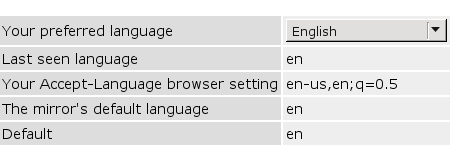
\includegraphics{cap03/language.png}
  \caption{Limba php.net}
  \label{fig:php.net lang}
\end{figure}
Setează-ţi şi următoarele preferinţe:
\begin{itemize}
\item \textbf{URL search fallback} -- Function list search
\item \textbf{Mirror site redirection} -- alege un mirror apropiat de locaţia ta geografică
\end{itemize}
Restul setărilor rămân la atitudinea ta.

Cu Firefox, mai poţi adăuga php.net şi ca motor de căutare, ca în
figura \ref{fig:php.net search}.

\begin{figure}[h!]
  \centering
    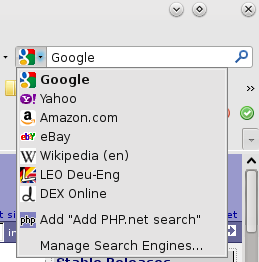
\includegraphics[width=150px]{cap03/search.png}
  \caption{Căutare în manualul PHP cu Firefox}
  \label{fig:php.net search}
\end{figure}

Introdu \textit{var\_dum}p în câmpul de căutare, şi vei fi condus
către pagina din manual a funcţiei. Acolo poţi vedea
în ordine
\begin{itemize}
\item versiunile PHP în care există funcţia
\item o descriere scurtă a funcţiei
\item semnătura funcţiei şi o descriere pe larg
\item eventuale avertizări
\item lista parametrilor şi semnificaţia lor
\item valoarea returnată
\item exemple de utilizare
\item funcţii înrudite
\item comentarii ale altor utilizatori
\end{itemize}
Sunt o grămadă de informaţii. Practic, manualul
PHP conţine toate informaţiile de care ai nevoie.
Din acest motiv cartea de faţă nu încearcă să 
duplice explicaţiile pe care le poţi găsi în manual,
ci doar să te călăuzească. În plus, comentariile
celorlalţi sunt extrem de utile. Foarte rar te vei
afla într-o situaţie unică în care nu s-a mai aflat
nimeni altcineva şi comentariile acelea nu îţi vor fi de 
folos. E recomandat să le citeşti şi pe ele.

\good{Cartea nu va explica toate funcţiile folosite
în listinguri. Când întâlneşti o funcţie nouă,
trebuie să te documentezi din manual.
}
\attention{Ceea ce ţi se va explica în carte sunt conceptele
generale şi termenii, astfel încât să te poţi
descurca singur.}

\subsection{Studiu de caz: funcţii variadice}
După cum observi în manual, funcţia \texttt{var\_dump()}
are de fapt semnătura
\begin{verbatim}
void var_dump (mixed $expression [, mixed $expression [, $... ]])
\end{verbatim}
\ldots înseamnă că funcţia acceptă un număr variabil
de parametri, însă trebuie să fie cel puţin unul.
Astfel de funcţii se numesc funcţii variadice (en. \textsl{variadic}).

\begin{Exercise}[title={Crează o funcţie variadică}]
\ExePart
Caută în manual funcţia \texttt{func\_num\_args()} şi
toate funcţiile înrudite cu ea pentru a crea
o funcţie variadică care returnează produsul parametrilor
pasaţi.

\ExePart
Scrie o nouă versiune a funcţiei care are semnătura
\begin{verbatim}
int array_product(array $numbers)
\end{verbatim}
şi care returnează produsul numerelor salvate în array.

% \ExePart
% 
% Ce observi? Cum poţi îmbunătăţi prima funcţie, cu respect
% faţă de a doua?
% TODO cum? nici eu nu mai ştiu
\end{Exercise}


\subsection{Categoriile de extensii disponibile}
Pe pagina oficială fiind, dacă navighezi către
\texttt{Documentation} $\rightarrow$ \texttt{View online}
$\rightarrow$ \texttt{English},
vei ajunge la indexul
manualului, la pagina sa de start.

Capitolele mari prezentate sunt lucruri precum
\textit{Getting Started} care conţine şi un tutorial,
\textit{Language Reference}, pe care l-ai
citit ca parte dintr-un exerciţiu din capitolul trecut,
\textit{Security} care conţine sfaturi de securitate,
şi asupra cărora vom reveni şi noi
în acest capitol, \textit{Features} îţi prezintă
unele capacităţi ale lui PHP folosite
în mod tipic de aplicaţii, \textit{PHP at the Core: A Hacker's Guide to the Zend Engine}
îţi prezintă inima interpreterului PHP, şi alte câteva capitole.

Deocamdată vrem să ne facem o imagine de ansamblu a funcţiilor
puse la dispoziţie, din capitolul \textit{Function Reference}.

\textit{Affecting PHP's Behaviour} sunt extensii care afectează
modul fundamental de funcţionare al lui PHP. De astfel de funcţii
nu vei avea nevoie decât când ajungi la nivelul avansat. Unele
dintre cele mai des folosite extensii din această categorie sunt
aşa numitele \textit{opcode cachers},
%TODO CHAP which chapter opcode cacher?
asupra cărora vom reveni într-un capitol viitor.

Extensiile pentru \textit{Audio Formats Manipulation} pun
la dispoziţie funcţii pentru formate audio de fişiere şi metadate
salvate în astfel de fişiere.

\textit{Authentication Services} sunt pentru servicii de autentificare,
utile în situaţii destul de complexe în care trebuie să integrezi
autentificarea utilizatorilor în alte servicii deja existente, sau să
faci autentificarea folosind servicii centralizate cu care şi alte aplicaţii pot
comunica.

\textit{Date and Time Related Extensions} conţin funcţii pentru
lucrul cu date şi timp, diferenţa dintre două date, convertirea
de input care reprezintă date sau timp în formate numerice uşor
de înţeles de către calculatoare\footnote{timestamps} sau fuse orare.

\textit{Compression and Archive Extensions} se ocupă de formate
de fişiere precum \texttt{zip} sau \texttt{phar},\footnote{php archive}
un format de arhivare propriu PHP care-ţi permite să incluzi aplicaţii
întregi dintr-un singur foc, chiar dacă acestea conţin câteva mii
de fişiere cu cod sursă.

\textit{Credit Card Processing} sunt pentru procesarea cărţilor de credit.

\textit{Cryptography Extensions} sunt utile atunci când vrei să
criptezi informaţii importante, precum numerele de conturi pe care le
procesezi cu funcţiile de procesare ale cărţilor de credit.

\textit{Database Extensions} pun la dispoziţie extensii pentru
comunicarea cu baze de date. MySQL este unul dintre cele mai folosite
sisteme de management al bazelor de date în aplicaţiile
PHP, însă există o grămadă de alte sisteme pentru organizarea
structurată a informaţiilor.

\textit{File System Related Extensions} se ocupă cu lucrul cu
fişiere şi directoare, citirea sau scrierea din/în fişiere,
listarea fişierelor dintr-un director, informaţii despre fişiere
precum drepturile de acces sau posesorii acestora.

\textit{Human Language and Character Encoding Support} sunt
printre altele pentru internaţionalizarea aplicaţiilor.
Dacă vrei să faci o aplicaţie cu interfaţa în mai multe
limbi, atunci trebuie să apelezi la funcţionalităţile
puse la dispoziţie de aceste extensii.

\textit{Image Processing and Generation} sunt pentru
prelucrarea şi generarea programatică a imaginilor.

\textit{Mail Related Extensions} sunt pentru
lucrul cu diferite protocoluri sau formate de e-mail.

\textit{Mathematical Extensions} pun la dispoziţie
funcţii matematice.

HTML este un limbaj bazat pe text.
\textit{Non-Text MIME Output} se ocupă cu
generarea de documente sau resurse în alte formate pe
lângă text precum animaţii flash sau documente PDF.

Funcţiile din extensiile de \textit{Process Control Extensions}
îţi permit să lansezi în execuţie alte programe cu interfaţă
CLI şi să
comunici cu acestea fie citind şi scriind din/în outputul/inputul
acelor procese, fie prin alte mecanisme precum IPC
(en. \textsl{inter-process communication}).

\textit{Other Basic Extensions} sunt extensii care pun
la dispoziţie diferite funcţionalităţi de bază.
Cele mai des întâlnite şi folosite sunt cele din
extensia \textit{URLs} şi din extensia \textit{Miscellaneous Functions}.

\textit{Other Services} conţine o mulţime de extensii. Una dintre
cele mai comune este \textit{sockets}. Cu ea poţi deschide
conexiuni programatic, aşa cum ai făcut cu telnet, şi transfera
date (în orice protocol, nu numai HTTP). Altă extensie folosită des
este \textit{cURL}, cu care poţi deschide conexiuni HTTP, fără
a fi nevoit să creezi manual cererile HTTP, aşa cum ai face-o cu
\textit{sockets}.

\textit{Search Engine Extensions} sunt extensii care te lasă
să comunici cu alţi daemoni care au menirea de a indexa
fişiere şi de a te lăsa să cauţi după cuvinte cheie de
exemplu. Majoritatea aplicaţiilor comune scrise în PHP
nu folosesc aceste servicii deoarece pentru aplicaţii mici
necesită prea multe resurse. Ele salvează datele în baze de
date, de obicei MySQL, şi caută manual. Aceste extensii
pentru \textit{search engine} sunt totuşi foarte
utile când vrei să faci ceva extensibil, fără a pune
presiune pe o bază de date. Ele reprezintă de fapt moduri "corecte"
de a implementa funcţionalitatea de căutare pe un site.

\textit{Server Specific Extensions} pun la dispoziţie
funcţii specifice SAPI-ului folosit. Dacă ai instalat
şi configurat mediul de programare ca în capitolul 1,
atunci foloseşti SAPI-ul Apache.

\textit{Session Extensions} pun la dispoziţie funcţionalitatea
numită \textsl{sesiuni}. Sesiunile permit aplicaţiilor web
să "ţină minte" utilizatorii şi date asociate cu aceştia.
Mulţumită sesiunilor este posibilă autentificarea utilizatorilor.

Categoria \textit{Text Processing} conţine extensii pentru
lucrul cu text, cu stringuri. Cele mai folosite extensii
din această categorie sunt \textit{Strings} pentru operaţii
cu stringuri precum căutare, stabilirea lungimii, ş.a.m.d.
şi \textit{PCRE} (en. \textsl{perl-compatible regular expressions}).
PCRE îţi permite să verifici dacă un string potriveşte o
regulă\footnote{Aşa cum ai inventat o regulă pentru
sintaxa limbajului HTML în capitolul 2} şi eventual
să şi extragi anumite secvenţe din acel string.\\
PCRE este puternic, dar consumă şi multe resurse,
deci este recomandat să foloseşti funcţiile simple
din extensia \textit{Strings} atunci când e posibil.

\textit{Variable and Type Related Extensions} pun
la dispoziţie funcţii pentru lucrul cu tipurile
de date fundamentale din PHP (în afară de stringuri,
care sunt tratate de extensiile prezentate anterior), printre
care array-uri, funcţii şi variabile. Atunci când ai căutat
informaţii despre funcţia \texttt{func\_num\_args()}
şi funcţiile înrudite cu ea, te-ai mişcat prin extensia
\textit{Function Handling}.

Extensiile din categoria \textit{Web Services} sunt folosite
pentru a crea şi folosi servicii web. Atunci când aplicaţia
ta pune la dispoziţie un serviciu web, aceasta poate
fi contactată de alte aplicaţii şi informaţiile pot
fi procesate programatic mult mai uşor. Acelaşi lucru îl
poţi face şi tu cu alte aplicaţii care îşi oferă
funcţionalităţile şi ca servicii web. De exemplu,
reţelele sociale precum Facebook\footnote{\url{http://facebook.com/}}
sau Twitter\footnote{\url{http://twitter.com/}} pun la dispoziţie
astfel de servicii. Asta le permite altor programatori să
creeze programe care postează tweet-uri pe twitter sau
jocuri pe care le poţi juca împreună cu prietenii tăi
pe facebook, aplicaţii care nu au legătură directă
cu firmele originale precum twitter sau facebook în
cazul nostru.

\textit{Windows Only Extensions} pun la dispoziţie funcţionalităţi
specifice Microsoft Windows. Acestea nu vor funcţiona decât dacă
daemonul cu PHP integrat în el rulează pe windows.
Este recomandat să nu foloseşti astfel de funcţii
decât în cazul în care ştii sigur că aplicaţia ta
va rula într-un mediu controlat, pe windows, deoarece
majoritatea serverelor rulează pe o formă sau alta
de *NIX\footnote{GNU/Linux, *BSD, SunOS, etc}, nu Windows.

\textit{XML Manipulation} pune la dispoziţie funcţionalitate
pentru lucrul cu fişiere în formatul XML. XML este un format
care-ţi permite să structurezi informaţii arborescente. Din punct
de vedere sintactic este
similar cu HTML, iar combinaţia dintre HTML şi XML a dat naştere
limbajului XHTML. În contrast cu (X)HTML însă, XML nu are
"taguri" predefinite. Programatorii îşi inventează
propriile formate de date şi le dau o semnificaţie.

Acestea au fost categoriile de extensii disponibile în PHP.
Unele dintre ele vin la pachet cu PHP, altele se află
în ceea ce numim PECL (en. \textsl{PHP Extension Community Library})
şi trebuie instalate separat.

Nu uita că deşi fac parte din aceeaşi categorie, două extensii nu
pot comunica una cu alta. De exemplu, dacă ai stabilit o conexiune
cu o bază de date MySQL, atunci nu poţi pasa această conexiune
unei funcţii care lucrează cu baze de date PostgreSQL. Cele două
extensii sunt complet diferite şi independente. Categorisirea
extensiilor este doar modul de organizare a informaţiilor în
manualul PHP, pentru o navigare mai uşoară.


\subsection{Extensii de bază}
În categoria \textit{Variable and Type Related Extensions}
este o extensie cu funcţii pentru lucrul cu array-uri.
Dacă urmezi link-ul \textit{Array Functions} vei vedea
indexul tuturor funcţiilor pentru array-uri alături de
o descriere scurtă a fiecăreia.

\begin{Exercise}[title={Înţelege manualul}]
Alege cinci funcţii de lucru cu array-uri şi
explică în cuvinte ce face fiecare, apoi crează
unul sau mai multe coduri sursă care să le demonstreze
utilitatea.
\end{Exercise}
\begin{Exercise}[difficulty=3,title={Explorează manualul}]
În acest moment ai o privire destul de robustă a
limbajului, dar nu ştii funcţiile care-ţi sunt
puse la dispoziţie. Totuşi, mulţumită explicaţiilor
de până acum, eşti capabil să înţelegi manualul.

Rezervă-ţi 40-80 de ore (1-2 săptămâni de lucru)
pentru a explora următoarele extensii:
\begin{itemize}
\item \textit{Array},
\textit{Function Handling}, \textit{Variable Handling} din categoria \textit{Variable and Type Related Extensions}
\item \textit{Strings} din categoria \textit{Text Processing}
\item \textit{Miscellaneous Functions} din categoria \textit{Other Basic Extensions}
\end{itemize}
Scrie scripturi de la simple la complexe care se folosesc
de aceste funcţii. Documentează-ţi scripturile cu comentarii.
La fiecare script scrie şi ce-ţi trece prin minte, ce observaţii
ai făcut, ce legături sau analogii ai făcut.

Nu uita să separi \textit{business logic} de \textit{view logic} şi să transmiţi date ce
rezultă în urma procesării formularelor (\textit{business logic}) către \textit{view logic}
folosind \textit{variabile intermediare}.

Postează fiecare cod sursă pe {\phpro} pentru a te verifica pe parcursul
celor 1-2 săptămâni, încă din momentul în care ai scris ceva nou.\footnote{Nu toate
scripturile deodată} În total ar trebui să ai câteva zeci bune de scripturi, cu
până la 1000 de LOCs sau chiar mai mult.

La fiecare exerciţiu explică modul de funcţionare \^in ceva asemănător cu
limbaj pseudocod, dar fără a folosi identificatori de variabile
sau a reflecta exact structura codului. Explică \^in schimb motivaţiile
de a proceda \^intr-un anumit fel.

Crează un jurnal al tuturor funcţiilor despre care te-ai documentat
singur din manual, cu semnătura funcţiei şi o explicaţie scurtă
despre ce face\footnote{Explicaţii scurte se pot găsi pe indexul
funcţiilor din manualul PHP.}.

După aceste 1-2 săptămâni nu îţi va mai sta nimic în calea creării
de site-uri destul de complexe {\ldots} cu câteva mici excepţii pe care le vom
aborda \^in cele ce urmează.
\end{Exercise}



%TODO ce altfel de explicaţii aş mai putea adăuga pentru a clarifica ev. nelămuriri?
%TODO pune-i pe cursanţi să înveţe din manual lucruri ca lucrul cu fs sau printf() & co şi observă dificultăţile





\section{Structuri de date}
Array-urile sunt atât de versatile încât pot fi folosite
pentru a construi structuri de date mai complicate, fiecare
cu avantajele şi dezavantajele sale.

\subsection{Stack şi queue}
Un \textsl{stack} este un array în care elementele sunt adăugate la sfârşit,
şi preluate tot de la sfârşit. Operaţia de adăugare a unui element
pe \textit{stack} se numeşte \textsl{push}, iar cea de scoatere se numeşte \textsl{pop}.

Un \textit{stack} poate fi reprezentat vizual ca în figura \ref{fig:stack}.

\begin{figure}[h!]
  \centering
    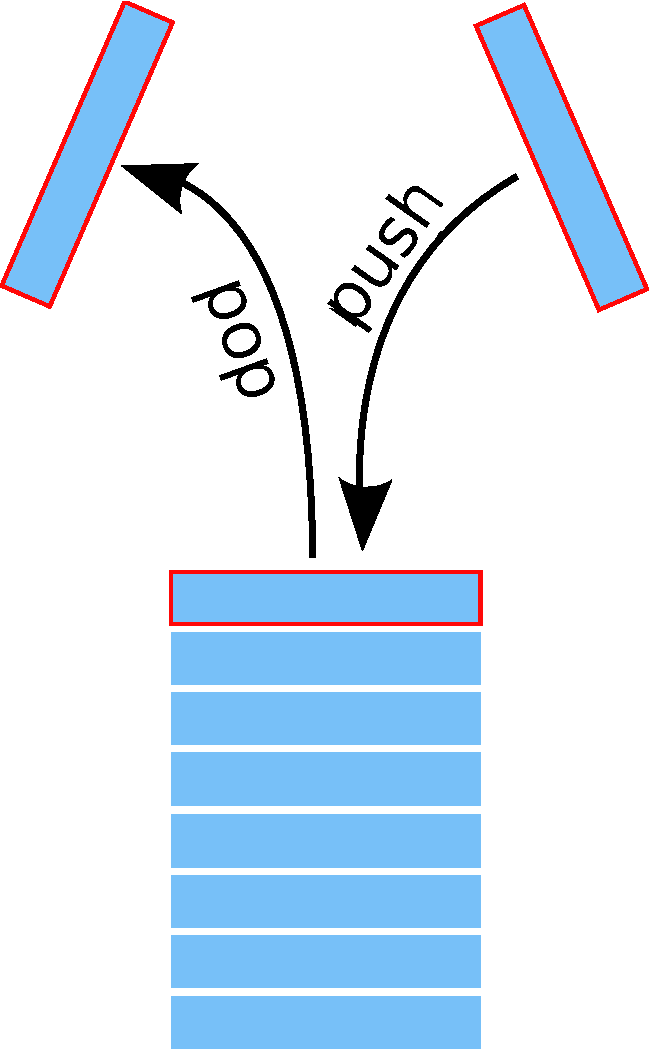
\includegraphics[scale=.3]{cap03/stack-crop.pdf}
  \caption{Operaţiile cu un stack}
  \label{fig:stack}
\end{figure}

Deoarece ultimul element adăugat este primul care este îndepărtat
din \textit{stack}, spunem că un \textit{stack} este o structură de date
de tip \textsl{LIFO} (en. \textsl{last in, first out}).

Operaţia \textit{push} îţi este cunoscută deja prin intermediul
operatorului \texttt{[]} pe care l-ai întâlnit în
listingul \ref{lst:push_operator}. Există şi o funcţie
absolut echivalentă în funcţionalitate cu acesta: \texttt{array\_push()}.

Similar cu LIFO, există şi FIFO (en. \textsl{first in, first out}),
numit şi \textsl{queue}. Operaţiile se numesc \textsl{shift} şi \textsl{unshift},
iar grafic ne putem imagina o astfel de structură de date ca în
figura \ref{fig:queue}.

\begin{figure}[h!]
  \centering
    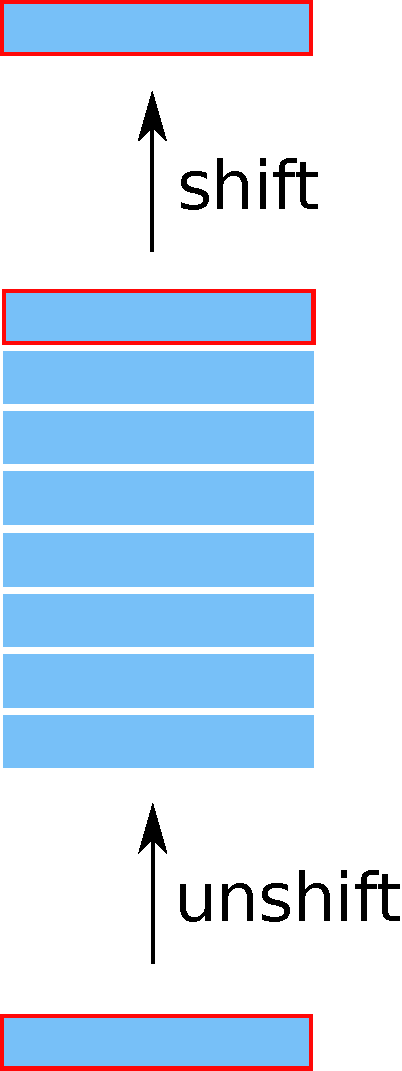
\includegraphics[scale=.3]{cap03/queue-crop.pdf}
  \caption{Operaţiile cu un queue}
  \label{fig:queue}
\end{figure}

Primul element pus în \textit{queue} este primul
element care va fi îndepărtat din \textsl{queue}.

Pentru aceste două operaţii există două funcţii numite
destul de intuitiv \texttt{array\_shift()} şi
\texttt{array\_unshift()}.



\begin{Exercise}[title={Experimentează cu stack şi queue}]
Scrie un script complet în care experimentezi cu
aceste structuri de date. Nu uita că poţi trata
acelaşi array alternativ, când ca \textit{stack}, când ca \textit{queue}.
\end{Exercise}

\subsection{Structuri de date recursive}
În exerciţiul \ref{ex:sintaxa_html} \textit{Sintaxa HTML} ai
făcut cunoştinţă cu recursivitatea. În PHP poţi procesa
structuri de date recursive folosind funcţii recursive.
De exemplu,
un document HTML este o structură de date recursivă
deoarece nodurile din
document\footnote{DOM - \href{http://en.wikipedia.org/wiki/Document_Object_Model}{document object model}}
pot avea în interiorul lor alte noduri. Din acest motiv
spunem că structurile de date recursive sunt şi izomorfice.

În capitolul trecut ai văzut cum poţi construi array-uri
n-dimensionale, unde n era bine determinat.

Un array recursiv este constituit, la fel ca şi un array
n-dimensional, din alte array-uri. Diferenţa este că
n nu este determinat. Trebuie să parcurgem recursiv
array-ul pentru a procesa fiecare element.

%TODO file cap03/family-tree* no longer needed

Vom lua ca exemplu un array recursiv:
\begin{lstlisting}
<?php
$arbore = array(
  'hello',
  'foo',
  'world' => array(
        'how',
        'are',
        'you',
        'today?' => array(
          'march',
          27,
          2010
        )
  ),
  'out',
  'there!'
);

foreach($arbore as $k => $v) {
  if(is_string($v)) {
	echo "$k => $v";
  }
  elseif(is_array($v)) {
	echo " *** RECURSIVITY";
  }
  echo PHP_EOL;
}
\end{lstlisting}
Practic nu este nimic nou. Iterăm array-ul şi afişăm
valorile. Însă pe linia 23 detectăm dacă valoarea însăşi
este la rândul ei tot un array (precum \texttt{\$arbore},
pe care tocmai îl iterăm), şi afişăm \texttt{" *** RECURSIVITY"}.

Ţin să subliniez: valoarea \$v este un array, şi chiar
dacă se află în interiorul unui array \$arbore, este tot un
array, deci \$v poate fi iterat cu exact aceeaşi buclă
\texttt{foreach}
cu care iterăm \$arbore.

Practic, nu trebuie decât să reutilizăm codul de pe liniile
19-27. Şi ce modalitate cunoaştem pentru a reutiliza codul?
Exact, funcţiile!

Deci implementăm o funcţie
\begin{verbatim}
void itereaza_recursiv(array $arbore)
\end{verbatim}
şi o apelăm, astfel:
\begin{lstlisting}
<?php
$arbore = array(
  'hello',
  'foo',
  'world' => array(
        'how',
        'are',
        'you',
        'today?' => array(
          'march',
          27,
          2010
        )
  ),
  'out',
  'there!'
);

function itereaza_recursiv($arbore) {
  foreach($arbore as $k => $v) {
        if(is_string($v) || is_numeric($v)) {
          echo "$k => $v";
          echo PHP_EOL;
        }
        elseif(is_array($v)) {
          echo "going into '$k'\r\n";
          itereaza_recursiv($v);
        }
  }
}

itereaza_recursiv($arbore);
\end{lstlisting}
După cum observi, funcţia \texttt{itereaza\_recursiv()} se apelează
pe ea însăşi pe linia 27, însă cu o altă valoare -- cu
valoarea elementului curent \$v, care este tot un array.
Pe linia 27 spunem că intrăm în recursivitate. La primul apel,
la elementul \texttt{'world'}, intrăm în adâncimea 1
a arborelui. În cadrul elementului \texttt{'world'}
se află încă un element la cheia \texttt{'today?'}
care are ca valoare un array. Atunci când se ajunge la el,
spunem că intrăm în adâncimea 2 "a recursivităţii".

După ce am afişat valoarea \texttt{2010}, ieşim din recursivitatea
de adâncime 2, revenind la 1, şi ne aflăm iar în array-ul cu
cheia \texttt{'world'}. Însă ajunşi aici, ne aflăm iar
la sfârşitul iteraţiei, deoarece bucla \texttt{foreach}
ajunge la sfârşitul array-ului salvat în elementul \texttt{'world'},
deci ieşim din recursivitate (şi deci din funcţia \texttt{itereaza\_recursiv()}),
revenind \ldots tot în funcţia \texttt{itereaza\_recursiv()}!

Însă acum ne aflăm pe linia 28, şi nu ne aflăm la sfârşitul recursivităţii
de "adâncime" 0, deci bucla foreach trece la următorul element: \texttt{'out'}.



\begin{Exercise}[title={Adâncimea recursivităţii},difficulty=2]
Modifică funcţia \texttt{itereaza\_recursiv()} dându-i semnătura:
\begin{verbatim}
string itereaza_recursiv(array $arbore, $depth=0)
\end{verbatim}
şi modifică implementaţia astfel încât fiecare afişare
de forma \texttt{"cheie => valoare"} să aibe în faţa sa
un număr de spaţii egal cu adâncimea din recursivitate la care
se află acel element, structura arborescentă fiind
astfel evidenţiată şi grafic:
\begin{verbatim}
0 => hello
1 => foo
going into 'world'
  0 => how
  1 => are
  2 => you
  going into 'today?'
    0 => march
    1 => 27
    2 => 2010
2 => out
3 => there!
\end{verbatim}
Funcţia nu trebuie să afişeze direct cu \texttt{echo},
ci să returneze outputul ca string, din motive
de modularizare.

Scriptul trebuie să funcţioneze ca script CLI,
nu printr-un daemon http, deci pentru a genera
o linie nouă în output foloseşte constanta
\texttt{PHP\_EOL}, pe care o cunoşti deja.
\end{Exercise}

Până acum am lucrat cu propriile structuri de date
recursive. Vei fi confruntat deseori cu necesitatea
de a inventa astfel de structuri de date, însă
şi mai des va trebui să procesezi date recursive
asupra cărora nu ai control. Un astfel
de exemplu este un director, căci un director poate avea
fişiere şi alte directoare în el. Observi recursivitatea?

Lucrul cu fişiere şi directoare se poate face
cu ajutorul extensiilor din categoria
\textit{File System Related Extensions}, mai exact
ne interesează în special extensia \textit{Directory Functions}.
Din extensia \textit{Filesystem Functions} avem nevoie
doar de funcţiile \texttt{is\_dir()} şi \texttt{is\_file()}
pentru a verifica dacă un element este director sau
fişier.

Începem prin doar a itera un director, fără
a intra recursiv în alte subdirectoare:

\begin{lstlisting}
<?php
function display_directory($dirpath) {
  $dh = opendir($dirpath);
  while($entry = readdir($dh)) {
	echo $entry;
	if(is_dir($dirpath.DIRECTORY_SEPARATOR.$entry)) {
	  echo DIRECTORY_SEPARATOR;
	}
	echo PHP_EOL;
  }
  closedir($dh);
}

display_directory(__DIR__);
\end{lstlisting}
\texttt{opendir()} ne returnează o resursă. Acesta este
un alt tip de date fundamental în PHP, însă
el nu poate fi creat direct de scripturile noastre,
ci doar prin intermediul funcţiilor native PHP,
implementate în extensii.

Deschizând un director cu \texttt{opendir()} avem
acces la această resursă şi îl putem itera.

Cu \texttt{readdir()} citim fiecare intrare din acest
director, salvând rezultatul în \texttt{\$entry}.
Această variabilă este fie un string, fie FALSE,
dacă am iterat totul, caz în care condiţia buclei
\texttt{while} va fi FALSE, deci se va ieşi din
bucla din fluxul de execuţie.

Pe linia 6 verificăm dacă noua intrare este un
director, şi dacă da, afişăm şi valoarea
constantă \texttt{DIRECTORY\_SEPARATOR}.
Diferite sisteme de operare folosesc diferite
separatoare în căile către fişiere şi directoare.
MS Windows foloseşte \texttt{\textbackslash}, în timp ce GNU/Linux
foloseşte \texttt{/}. Constanta \texttt{DIRECTORY\_SEPARATOR}
va avea mereu valoarea corespunzătoare platformei
pe care rulează scriptul.

Afişarea acestei
constante este doar un indiciu vizual pentru noi,
să ştim dacă avem de-a face cu un fişier, sau cu un
director. În practică, aici ar trebui să
intrăm recursiv în noul subdirector.

Toate\footnote{Aproape toate} directoarele
au două pseudo-directoare în ele: \texttt{'.'}
şi \texttt{'..'}. Acestea nu sunt directoare
în adevăratul sens al cuvântului, ci sunt referinţe,
primul către directorul însuşi, al doilea către
directorul părinte. Cu siguranţă ai folosit
deja în HTML căi relative precum
\begin{lstlisting}[language=HTML]
<img src="../img/me.jpg">
\end{lstlisting}
De aici vine acel \texttt{'..'}.

\begin{Exercise}[title={Determinarea recursivă a conţinutului unui director},difficulty=2]
În funcţia anterioară, în loc de simpla afişare
a valorii \texttt{DIRECTORY\_SEPARATOR}, vrem să intrăm în
directorul respectiv. Extinde şi modifică funcţia
astfel încât să aibe semnătura
\begin{verbatim}
array get_directory_structure(string $dir_path)
\end{verbatim}
şi să returneze fişierele şi toate subdirectoarele din
directorul \$dir\_path într-un array recursiv.
\end{Exercise}

\begin{Exercise}[title={Afişarea unei structuri de date recursive},difficulty=1]
\ExePart

Implementează o funcţie
\begin{verbatim}
string render_recursive_array_to_ul(array $array)
\end{verbatim}
care acceptă ca parametru un array (eventual recursiv) şi returnează
reprezentarea HTML a acestuia într-o listă neordonată (\texttt{<ul>}).

Acestei funcţii îi vei putea pasa valoarea returnată
de un apel la \texttt{get\_directory\_structure()} implementată
în exerciţiul anterior.

Observi cum implementaţia de funcţii care operează
doar pe date abstracte (aici: array-uri) duc
automat la reutilizarea şi o mai bună
modularizare a codului?

\ExePart

Extinde funcţia astfel încât să accepte şi o funcţie anonimă
ca \textit{callback}:
\begin{verbatim}
string render_recursive_array_to_ul(array $array,callback $cb=NULL)
\end{verbatim}
care dacă este prezent, este folosit pentru a genera outputul
ce trebuie pus între \texttt{<li>} şi \texttt{</li>}.
Semnătura callback-ului trebuie să fie
\begin{verbatim}
string cb(string $path)
\end{verbatim}
\end{Exercise}

\section{Call Stack}
Atunci când apelăm o funcţie, PHP pune contextul actual de execuţie
pe un stack (operaţia \textit{push}), şi apoi se apelează funcţia.
La ieşirea din funcţie (cu un \texttt{return}), PHP face un
\textit{pop} pentru acel stack, şi execuţia se continuă de unde
fusese întreruptă anterior.

Acest stack se numeşte \textsl{call stack}, fiecare element
de pe acest stack fiind numit \textsl{call frame}.
\section{Fişiere multiple}
Până acum ne-am structurat scripturile în funcţii reutilizabile pe de o parte,
şi pe de alta separând \textit{business logic} de \textit{view logic}, însă
totul se afla într-un singur fişier. Nu puteam refolosi nici logica, nici
prezentarea, separate una de alta.

PHP ne pune la dispoziţie patru directive pentru includerea unui fişier în
alt fişier .php. Primele două se numesc \texttt{include} şi \texttt{require}.
Sintaxa este destul de intuitivă:
\begin{verbatim}
include <string>;
require <string>;
\end{verbatim}

Exemplu:
\begin{lstlisting}[title=index.php]
<?php
if(isset($_GET['nume']) && is_string($_GET['nume'])) {
  $nume = $_GET['nume'];
}

if(isset($nume)) {
  include 'greet_nume.php';
}
include 'greeting_form.php';
\end{lstlisting}
\begin{lstlisting}[title=greet\_nume.php]
Salut <?php echo $nume; ?>.
\end{lstlisting}
\begin{lstlisting}[title=greeting\_form.php,language=html]
<form method="GET" action="index.php">
  <input type="text" name="nume" />
  <input type="submit" value="greet" />
</form>
\end{lstlisting}

Bineînţeles exemplul nostru nu este atât de complex încât 
avantajele să devină evidente. Un avantaj posibil ar fi că putem schimba modul
de funcţionare extrem de uşor, fără a modifica nici un alt
fişier în afara lui \texttt{index.php}.

Aşa cum este acum, scriptul afişează formularul indiferent
dacă avem numele ca input sau nu. Am putea schimba rapid în afişarea
formularului doar dacă numele nu a fost trimis de utilizator, modificând
\texttt{index.php} astfel:
\begin{lstlisting}[title=index.php,firstnumber=6]
if(isset($nume)) {
  include 'greet_nume.php';
}
else {
  include 'greeting_form.php';
}
\end{lstlisting}
fără a ne atinge de nici un alt fişier.

Alt avantaj e că am putea refolosi \texttt{greet\_nume.php} oricând
vrem să salutăm pe cineva. Nu ar trebui decât să ne asigurăm că există variabila
\texttt{\$nume}, deoarece aceasta este folosită de acel script.

Diferenţa dintre \texttt{include} şi \texttt{require} constă în cum
tratează PHP absenţa fişierului inclus. Cu \texttt{include}, PHP generează
o avertizare dar continuă execuţia. Cu \texttt{require}, execuţia se opreşte
complet dacă fişierul nu există sau PHP nu îl poate citi. De aceea,
este recomandat să folosim \texttt{require} atunci când ştim că aplicaţia
nu ar avea oricum să-şi îndeplinească (măcar parţial) execuţia fără
fişierul php pe care vrem să-l injectăm în runtime-ul php.

\attention{Sub MS Windows, \textbackslash trebuie precedat de un alt \textbackslash
în stringurile interpolate atunci când sunt declarate căi pentru filesystem.}

Celelalte două directive pentru includerea codului de fişiere este familia
\texttt{*\_once}. Sintaxa:
\begin{verbatim}
include_once <string>;
require_once <string>;
\end{verbatim}
Aşa cum le spune şi numele, aceste constructe vor include fişierul doar o singură
dată. Asta este foarte util dacă fişierul inclus conţine implementările unor funcţii,
deoarece, dacă am implementa o funcţie cu acelaşi nume de mai multe ori, PHP
ne-ar spune că nu putem redeclara acea funcţie. Exemplu:
\begin{lstlisting}
<?php
include_once 'functions.php';
include_once 'functions.php';//nu va mai fi inclus inca o data
echo foo();
\end{lstlisting}
Unde funcţia \texttt{foo()} este implementată în fişierul \texttt{functions.php}.
Totuşi în acest caz ar fi mai bine să folosim \texttt{require\_once}, astfel încât dacă
fişierul \texttt{functions.php} nu există, execuţia să fie întreruptă din start.
Nu are rost să încercăm să executăm un cod care apelează o funcţie care nu există,
deoarece fişierul în care ar trebui să fie implementată nu există.

\subsection{Şabloane}
În exemplul anterior, \texttt{greet\_nume.php} se numeşte \engl{şablon}{template}.
Folosirea lui este însă dependentă de existenţa unei variabile numită \texttt{\$nume},
ceea ce face \textit{template}-ul nostru să fie cuplat de această variabilă, la fel
cum şi cuvântul cheie \texttt{global} cuplează numele unei variabile de o funcţie.

Putem decupla foarte elegant orice template de variabilele folosite
în el creând o funcţie precum:
\begin{verbatim}
void render(string $template, array $vars=NULL)
\end{verbatim}
unde \texttt{\$template} este calea către un fişier .php folosit
ca template, iar \texttt{\$vars} este un array asociativ. Acest array
va fi iterat ca în listingul \ref{lst:varvarfromassoc}, creând astfel
variabilele cerute de template-ul \texttt{\$template}. Aceste variabile
vor fi locale funcţiei \texttt{render()},\footnote{Se vor afla doar în scope-ul local
al funcţiei} deci nu vor polua nici un scope, fiind şterse automat de PHP
atunci când fluxul de execuţie iese din funcţie. În acelaşi timp, variabilele
specifice template-ului nu vor fi cuplate de \textit{scope}-ul global, aşa cum \texttt{\$nume}
folosit de \texttt{greet\_nume.php} era cuplat de \texttt{\$nume} din \textit{scope}-ul
global (\texttt{index.php}).

După ce variabilele variabile
au fost create, o simplă instrucţiune de includere a fişierului va genera outputul.

Dacă funcţia nu primeşte un al doilea parametru de la apelant, atunci \texttt{\$vars}
va avea valoarea \texttt{NULL}, şi nu ar trebui să mai creăm variabilele variabile,
ci doar să includem \textit{template}-ul.

\begin{Exercise}[title={O funcţie render()}]
\ExePart
Scrie o funcţie
\begin{verbatim}
void render(string $template, array $vars=NULL)
\end{verbatim}
care crează variabile variabile pe baza array-ului asociativ \$vars
şi apoi include \$template.

Exemplu de apelare a acestei funcţii:
\begin{lstlisting}
render('greet_nume.php',array('nume' => $nume));
\end{lstlisting}

\ExePart

Rescrie funcţia \texttt{render()} folosind funcţia internă
\texttt{extract()}.
%TODO WIKI: explică ce e o funcţie internă şi că trebuie înlocuit cu foreach
\end{Exercise}
În exemplul din exerciţiul anterior am apelat funcţia cu parametrul
\texttt{array('nume' => \$nume)}. În PHP există funcţia \texttt{compact()}
care poate crea un array asociativ cu numele variabilelor ca chei, şi
valorile acestora ca valori în array. Este o funcţie foarte utilă
atunci când numele variabilelor din \textit{scope}-ul actual (în cazul de
faţă cel global) sunt numite la fel ca variabilele folosite în
\textit{template}-ul în cauză.


\subsection{Primul site complet}
Hai să vedem cum putem folosi toate lucrurile învăţate sau nu până acum. Includ
şi lucrurile neînvăţate, deoarece mă aştept să te documentezi din manual
atunci când întâlneşti o funcţie necunoscută.

O vom lua gradual, adăugând treptat funcţionalitate, şi deci şi complexitate.

Vrem să facem un site personal cu câteva pagini. Întregul site va prezenta
pe toate paginile un meniu comun cu lista paginilor existente. 

\begin{figure}[H]
  \centering
    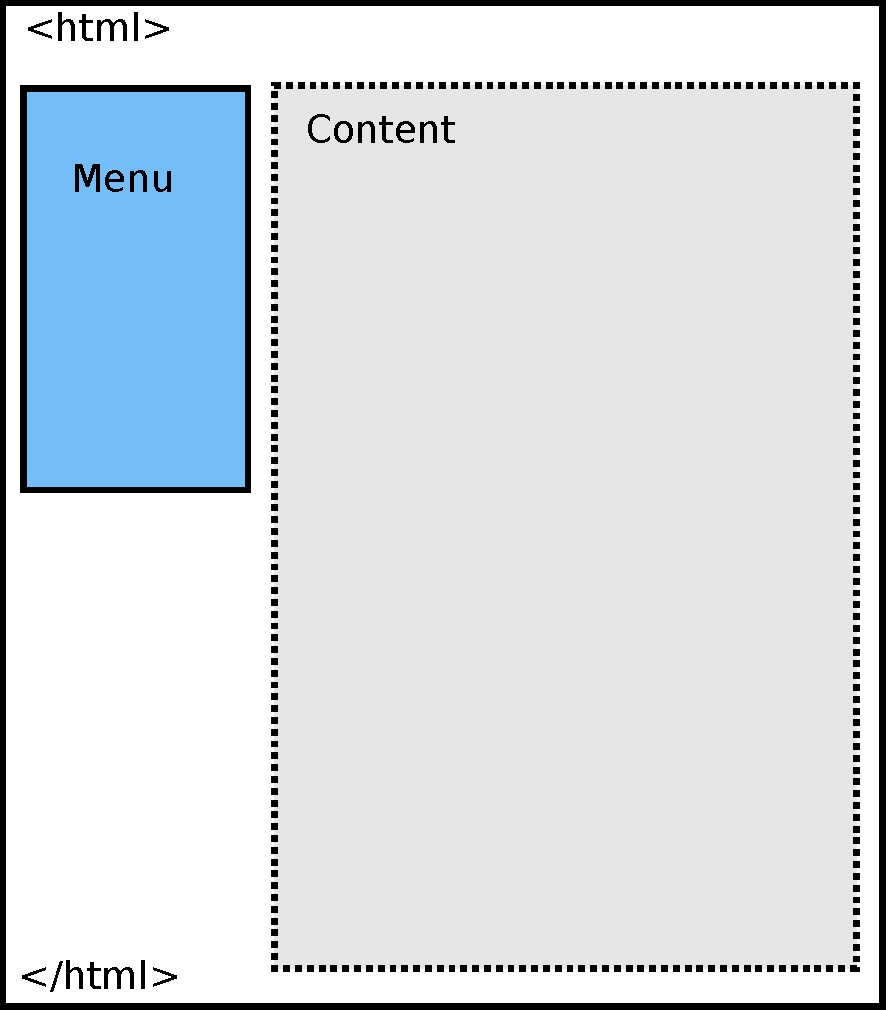
\includegraphics[scale=.5]{cap03/homepage-layout-crop.pdf}
  \caption{Layout site personal}
  \label{fig:layout site personal}
\end{figure}

Toate paginile vor
arăta similar, doar conţinutul efectiv al fiecărei pagini fiind diferit. Spunem că site-ul
foloseşte un \textit{template}. Acesta va arăta ca în figura \ref{fig:layout site personal}.


\begin{Exercise}[title={Crează template}]
Crează un fişier XHTML 1.1 structurat ca
în figura \ref{fig:layout site personal}. Alegerea culorilor şi aşezarea
în pagină sunt lăsate la atitudinea ta, dar meniul trebuie să fie
definit aşa:
\begin{lstlisting}[language=html]
<div id="menu">

</div>
\end{lstlisting}
iar continutul aşa:
\begin{lstlisting}[language=html]
<div id="content">

</div>
\end{lstlisting}
\end{Exercise}

Pentru site-ul nostru,
am fi tentaţi să punem acest \textit{template} în \texttt{index.php}.
Asta nu ar fi o decizie bună, deoarece nu am putea reutiliza \textit{template}-ul
în alte locuri. \texttt{index.php} ar trebui doar să coordoneze
conlucrarea dintre \textit{business logic} şi \textit{view logic}.
Deci pune template-ul creat într-un fişier nou numit \texttt{layout.php}.
Acum creăm şi index.php, care va afişa template-ul. Ulterior urmează să adăugăm
şi procesările (\textit{business logic}) corespunzătoare:
\begin{lstlisting}[title=index.php]
<?php
require_once 'functions.php';
//here be processing

render('layout.php');
\end{lstlisting}
Crează şi fişierul \texttt{functions.php} şi pune
în el implementaţia funcţiei \texttt{render()} creată
în unul din exerciţiile anterioare.

Acum hai să facem layout-ul să folosească câteva variabile:
\texttt{\$title}, \texttt{\$menu}, şi \texttt{\$content}.
Înlocuieşte astfel încât să ajungi la:
\begin{lstlisting}[numbers=none]
<title><?php echo $title;?></title>
\end{lstlisting}
\begin{lstlisting}[numbers=none]
<div id="menu"><?php echo $menu;?></div>
\end{lstlisting}
şi
\begin{lstlisting}[numbers=none]
<div id="content"><?php echo $content;?></div>
\end{lstlisting}

Deoarece \textit{template}-ul foloseşte acum aceste
variabile, trebuie să i le exportăm. Deci adaugă
un array asociativ corespunzător:
\begin{lstlisting}[title=index.php]
<?php
require_once 'functions.php';
$tpl_vars = array(
  'title' => 'My Homepage',
  'menu' => 'no menu yet',
  'content' => 'no content yet'
);

render('layout.php',$tpl_vars);
\end{lstlisting}

Însă am spus că vrem să afişăm diferite pagini, fiecare pagină cu conţinutul ei, şi
în plus fiecare pagină să aibe un link în meniu.

Cu siguranţă ne-am putea apuca să mâzgălim nişte cod la grămadă, şi cu siguranţă
ne va ieşi ceva aspectuos. Dar cel mai probabil nu ne va ieşi ceva reutilizabil
dacă nu stăm să ne gândim puţin mai profund şi mai sistematic de ce avem nevoie.

Încă o dată, rezumăm: o pagină are
\begin{itemize}
\item un titlu, pus în <title></title> în template
\item un conţinut
\item un meniu
\end{itemize}
În exemplul de mai sus, conţinutul este la noi un string. Însă acest conţinut
va diferi de la pagină la pagină, şi cel mai probabil va fi foarte lung.

Am putea teoretic să punem conţinutul fiecărei pagini într-un string, însă
asta ar face codul foarte greu de citit şi mentenat. Mult mai curat ar fi
dacă am considera un nume de fişier ca fiind caracteristica "conţinut"
a acelei pagini. Altfel spus, o pagină ar consista din:
\begin{itemize}
\item un titlu, pus în <title></title> în template
\item un fişier cu conţinutul efectiv
\item un meniu
\end{itemize}
Deci am putea crea o structură de date abstractă care să conţină o pagină.
Deoarece avem o serie de trei caracteristici pentru o pagină, putem
salva aceste informaţii despre fiecare pagină într-un array asociativ:
\begin{lstlisting}
$home = array(
  'title' => 'Bine ai venit',
  'content' => 'home.php',
  'menu' => 'no menu yet'
);
$about = array(
  'title' => 'Despre mine',
  'content' => 'despre.php',
  'menu' => 'no menu yet'
);
\end{lstlisting}
Nu m-am grăbit să creez şi meniul pentru fiecare pagină, deoarece
am realizat că acest meniu ar putea fi determinat programatic, pe baza
variabilelor precum \texttt{\$home} sau \texttt{\$about}. Ce ar implica
generarea automată a meniului pentru fiecare pagină? Exact! Ar
implica iterarea acestor variabile. Însă noi nu putem itera variabile.
Putem itera array-uri. De aici ne vine ideea genială de a salva toate
paginile într-un array asociativ. 
Hai să vedem cum va arăta \texttt{index.php}

\begin{lstlisting}
<?php
require_once 'functions.php';

$pages = array(
  'home' => array(
	'title' => 'Bine ai venit',
	'content' => 'home.php',
	'menu' => 'no menu yet'
  ),
  'about' => array(
	'title' => 'Despre mine',
	'content' => 'despre.php',
	'menu' => 'no menu yet'
  )
);

$tpl_vars = array(
  'title' => 'My Homepage',
  'menu' => 'no menu yet',
  'content' => 'no content yet'
);

render('layout.php',$tpl_vars);
\end{lstlisting}
Realizăm două lucruri:
\begin{itemize}
\item variabila \texttt{\$tpl\_vars} devine inutilă -- toate informaţiile se află acum în \texttt{\$pages},
chiar dacă nu în exact aceeaşi formă. De exemplu, va trebui să găsim o metodă de a "citi" fişierul .php
cu conţinutul, deoarece nu vom mai avea la dispoziţie conţinutul efectiv ca string
\item variabila \texttt{\$pages} este ca un fel de \textit{variabilă de configurare}.
Atunci când am separat \textit{business logic} de \textit{view logic},\footnote{folosind
funcţia proprie \texttt{render()}} am spus că misiunea lui \texttt{index.php} este să
coordoneze conlucrarea dintre diferite componente, deci deşi este posibil să
punem configuraţiile într-un astfel de script "de coordonare", mult mai curat ar fi
să separăm şi configurarea de celelalte două procese izolate, şi anume \textit{business logic}
şi \textit{view logic}
\end{itemize}
Pentru primul punct avem puţin mai mult de muncă, dar pentru al doilea există o soluţie
foarte elegantă. Familia de directive \textit{include} nu numai că include
un fişier, dar şi este evaluat ca valoarea returnată de fişierul inclus.\footnote{Astfel
de detalii, dar multe altele, pot fi citite în manualul PHP, capitolul
\textit{Language Reference}} Astfel
am putea avea un fişier de configurare \texttt{pages.php}:
\begin{lstlisting}[title=pages.php]
<?php
return array(
  'home' => array(
	'title' => 'Bine ai venit',
	'content' => 'home.php'
  ),
  'about' => array(
	'title' => 'Despre mine',
	'content' => 'despre.php'
  )
);
\end{lstlisting}
Iar index-ul nostru va deveni mult mai curat:
\begin{lstlisting}
<?php
require_once 'functions.php';
$pages = require_once 'pages.php';

render('layout.php');
\end{lstlisting}

Pentru a afişa diferite pagini, nu trebuie decât să acceptăm un
parametru prin \texttt{\$\_GET} în funcţie de care să
decidem care dintre pagini trebuie afişată.

Vom modifica corespunzător \texttt{index.php}:

\begin{lstlisting}[title=index.php]
<?php
require_once 'functions.php';
$pages = require_once 'pages.php';

if(isset($_GET['show']) && array_key_exists($_GET['show'], $pages)) {
  $page = $_GET['show'];
}
else {
  $page = 'home';
}

render('layout.php',$pages[$page]);
\end{lstlisting}
Însă asta ne va afişa ca conţinut numele fişierelor, nu conţinutul acelor
fişiere, care nici măcar nu există încă.

Deci crează mai întâi un subdirector \texttt{pages} şi în el două fişiere
\texttt{home.php} şi \texttt{despre.php} cu un conţinut HTML
la alegere. Apoi modifică layout-ul astfel încât să includă fişierul
pe care-l primeşte în variabila \texttt{\$content}, în loc să îl afişeze
direct:
\begin{lstlisting}[numbers=none,language=html]
<div id="content">
<?php include __DIR__ . '/pages/' . $content; ?>
</div>
\end{lstlisting}

Un ultim lucru mai avem de făcut: să construim meniul dinamic,
pe baza informaţiilor din \texttt{\$pages}. Membrul \texttt{'menu'}
al fiecărei pagini din \texttt{\$pages} nu îşi are rostul, constituie
doar informaţii redundante ce pot fi deduse din \texttt{\$pages}.

Deci vom crea o funcţie care ia ca parametru un array precum \texttt{\$pages}
şi generează un meniu HTML. Deoarece o astfel de funcţie
are rol ajutător, şi în fapt marginal funcţionării aplicaţiei
dincolo de formatul HTML, numim o astfel de funcţie un \textsl{helper}.
Funcţia va avea semnătura:
\begin{verbatim}
string build_menu_from_pages(array $pages)
\end{verbatim}
Implementaţia o adăugăm în fişierul \texttt{functions.php}
\begin{lstlisting}[numbers=none,title=functions.php]
function build_menu_from_pages($pages) {
  $r = '<ul>';
  foreach($pages as $pagename => $metadata) {
	$r .= '<li><a href="?show='.$pagename.'">'.$metadata['title'].'</a></li>';
  }
  return $r.'</ul>';
}
\end{lstlisting}

Felicitări. Acum nu numai că ai un site, dar ai o structură
flexibilă pe a cărei fundaţie poţi adăuga uşor pagini noi.
Pentru a adăuga o pagină nouă de exemplu, tot ce trebuie
să faci este să o creezi în subdirectorul \texttt{pages}
şi să o înregistrezi ca pagină validă în \texttt{pages.php},
alături de metadate despre pagină precum titlul paginii.
În rest, nu trebuie să te atingi de nici un alt cod,
nu trebuie să muţi sau să editezi cod, iar meniul va fi
construit automat.

Pentru recapitulare, figura \ref{fig:filestruct-homepage}
prezintă încă o dată structura de fişiere creată
şi scopurile lor.

\begin{figure}[H]
  \centering
    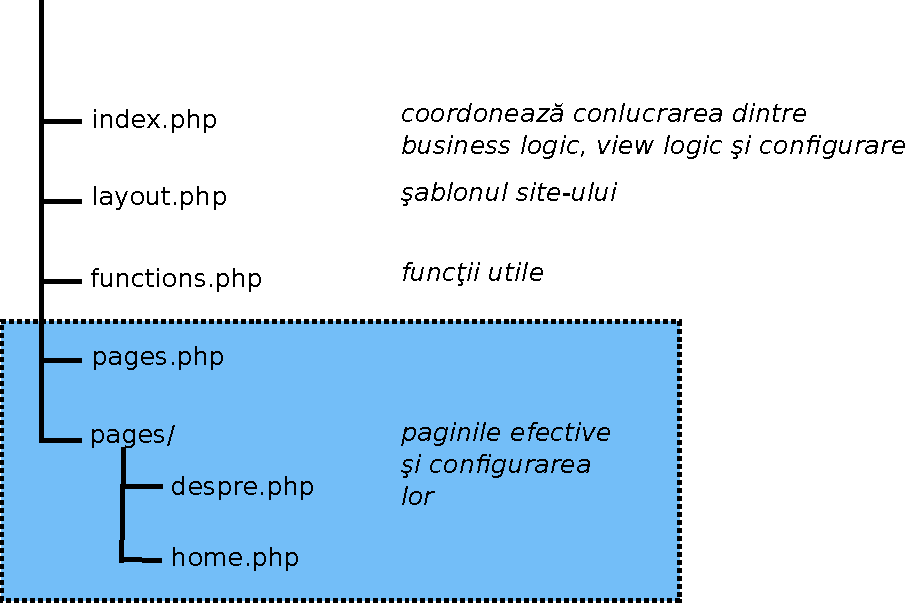
\includegraphics[scale=.5]{cap03/structure-homepage-crop.pdf}
  \caption{Structura fişierelor unui site simplu}
  \label{fig:filestruct-homepage}
\end{figure}

\begin{Exercise}[title={Îmbunătăţeşte-ţi pagina personală},difficulty=1]
\ExePart
Momentan meniul conţine link  si pentru pagina activă,
ceea ce nu prea are sens. Extinde funcţia
\texttt{build\_menu\_from\_pages} astfel încât să
nu genereze link pentru pagina activă momentan, ci
doar să o afişeze în lista neordonată ca text.

\ExePart
\texttt{index.php} conţine \textit{business logic}-ul site-ului tău.
Extinde acest \textit{business logic} astfel încât pentru
paginile inexistente să arate o pagină \texttt{notfound.php}.
\texttt{home.php} trebuie să rămână în continuare pagina de
start standard a site-ului.

\ExePart
Adaugă încă o pagină \textit{Despre tine}
care afişează informaţii despre vizitator din array-ul superglobal
\texttt{\$\_SERVER}.

Dacă ştii CSS, stilizează site-ul aşa încât să fie mai aspectuos.
Nu va trebui să modifici în nici un fel layout-ul sau
paginile individuale. Vei lucra doar cu CSS.
%TODO wiki: posibilă greşeală: folosirea $_SERVER direct în view
\end{Exercise}

Din partea I a exerciţiului se observă în practică un alt avantaj
al funcţiilor: nu trebuie să editezi multe fişiere în lungul
şi-n latul proiectului, nu te atingi de \textit{business logic}
sau de \textit{view logic} deoarece nu modifici modul fundamental de funcţionare
al acestora. Doar îmbunătăţeşti funcţia, iar
modificările sunt preluate automat în toate locurile de unde
aceasta este apelată.

\section{Directorul curent de lucru}
Căile relative către fişiere şi directoare,
sunt relative la ceea ce numim \textsl{current working
directory}. La \textsl{runtime} (în timpul execuţiei
scriptului), putem afla CWD-ul cu
funcţia \texttt{getcwd()}, şi schimba CWD-ul cu \texttt{chdir()}.

În exemplele anterioare, instrucţiuni precum
\begin{lstlisting}
<?php
require_once 'functions.php';
\end{lstlisting}
au funcţionat deoarece directorul curent de lucru \texttt{'.'}
este specificat în mod standard în directiva \texttt{php.ini}
\texttt{include\_path}. Modul corect de a include un fişier, fără
a ne baza pe faptul că acesta se află în \texttt{include\_path}, ar fi
\begin{lstlisting}
<?php
require_once './functions.php';
\end{lstlisting}
unde \texttt{'.'} se referă la CWD.

Dacă avem însă un scenariu mai complex, cu următoarele fişiere:
\begin{figure}[h!]
  \centering
    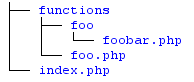
\includegraphics[scale=.7]{cap03/cwdtree.png}
  \caption{Scenariu includere}
  \label{fig:cwdtree}
\end{figure}

\begin{lstlisting}[title=index.php]
<?php
require_once './functions/foo.php';

echo 'index.php este in directorul ',__DIR__,PHP_EOL;

echo 'apelul la foo() genereaza:';
foo();
echo PHP_EOL;
\end{lstlisting}

\begin{lstlisting}[title=functions/foo.php]
<?php
require_once './foo/foobar.php';
function foo() {
        echo __DIR__;
}
\end{lstlisting}

\begin{lstlisting}[title=functions/foo/foobar.php]
<?php
function foobar() {
}
\end{lstlisting}

Toate fişierele sunt incluse prin prisma fişierului
\texttt{index.php}, deci CWD-ul este directorul
în care se află acest fişier. Asta nu este
o problemă pentru linia 2 din \texttt{index.php},
deoarece directorul \texttt{'.'} coincide
cu directorul în care se află \texttt{index.php}.

Însă devine o problemă atunci când din fişierul
inclus \texttt{foo.php} vrem să includem
un alt fişier dintr-un alt subdirector
\texttt{functions/foo/}, deoarece CWD-ul nu se
schimbă, şi deci, relativ la directorul
în care se află \texttt{index.php}, nu există
un subdirector \texttt{./foo/foobar.php}.

O metodă foarte elegantă la problema asta este să definim
o constantă în \texttt{index.php}, constantă care
va fi folosită la includerea fişierelor. Astfel am
avea:

\begin{lstlisting}[title=index.php]
<?php
const APP_ROOT = __DIR__;
require_once APP_ROOT . '/functions/foo.php';

echo 'index.php este in directorul ',__DIR__,PHP_EOL;

echo 'apelul la foo() genereaza:';
foo();
echo PHP_EOL;
\end{lstlisting}

\begin{lstlisting}[title=functions/foo.php]
<?php
% require_once APP_ROOT . '/functions/foo/foobar.php';
function foo() {
        echo __DIR__;
}
\end{lstlisting}
Cu această tehnică vom avea în lungul şi-n latul
aplicaţiei constanta \texttt{APP\_ROOT} care
conţine mereu calea către directorul în
care se află în \texttt{index.php}, indiferent
de fişierul prin care trece momentan fluxul
de execuţie.

Cu adevărat flexibilă devine această metodă
atunci când avem aplicaţii multiple care
folosesc un set comun de funcţii. Nu va trebui
să copiem fişierele de colo colo, ci vom
dezvolta doar o singură "versiune" a acestor
funcţii comune, definind o constantă 
de genul \texttt{APP\_LIB} cu calea către
directorul ce conţine fişiere PHP
cu implementările funcţiilor noastre. Din a doua aplicaţie
care doreşte să folosească funcţiile primei
aplicaţii, nu trebuie decât să definim
\texttt{APP\_LIB} ca calea către
directorul cu funcţii din prima aplicaţie,
cea "originală".

Şi mai curat din punct de vedere organizatoric
este să punem toate aceste funcţii într-o
locaţie neutră, astfel încât să nu aparţină
nici unui proiect, şi din toate
proiectele să definim calea către acea
locaţie.

O altă tehnică implică folosirea tocmai
a acestei constante magice  \texttt{\_\_DIR\_\_}.

Cu această tehnică nu mai e nevoie
să definim constante "globale" precum \texttt{APP\_ROOT},
însă nici nu mai putem reutiliza porţiuni
de funcţionalitate în lungul şi-n latul
diferitelor proiecte independente unul de celălalt.

Un astfel de cod ar arăta astfel:
\begin{lstlisting}[title=index.php]
<?php
require_once './functions/foo.php';
foo();
\end{lstlisting}

\begin{lstlisting}[title=functions/foo.php]
<?php
require_once __DIR__ . '/foo/foobar.php';
function foo() {
}
\end{lstlisting}

\begin{lstlisting}[title=functions/foo/foobar.php]
<?php
function foobar() {
}
\end{lstlisting}

\section{Formulare II. File uploads}
Cu PHP, poţi oferi utilizatorului posibilitatea de a salva fişierele
proprii pe hard disk-ul serverului. Este ceea ce numim \textsl{file upload}.

Formularele care conţin câmpuri pentru upload trebuie să fie trimise
cu metoda HTTP POST, şi să fie codate ca \texttt{multipart/form-data}.

Un exemplu:
\begin{lstlisting}[title=index.php]
<?php
require_once __DIR__ . '/functions.php';

echo '<pre>';
var_dump($_FILES);
echo '</pre>';
?>
<form enctype="multipart/form-data" method="POST">
<input type="hidden" name="MAX_FILE_SIZE"
	value="<?php echo return_bytes(ini_get('upload_max_filesize'));?>" />
<input name="myfile" type="file" />
<input type="submit" value="Send" />
</form>
\end{lstlisting}

\begin{lstlisting}[title=functions.php]
<?php
function return_bytes($val) {
  $val = trim($val);
  $last = $val[strlen($val)-1];
  switch($last) {
	case 'g':
	case 'G':
	  $val *= 1024;
	case 'm':
	case 'M':
	  $val *= 1024;
	case 'k':
	case 'K':
	  $val *= 1024;
  }
  return $val;
}
\end{lstlisting}
Codul este destul de sugestiv. La primirea fişierelor (cu succes sau cu erori, nu
contează), informaţiile\footnote{metadatele} despre ele vor fi disponibile
în array-ul superglobal \texttt{\$\_FILES}.

Elementul \texttt{'error'} din fiecare set de metadate va conţine
codurile de eroare pe care le poţi compara
cu constantele specifice\footnote{\url{http://www.php.net/manual/en/features.file-upload.errors.php}}
pentru a determina cauza erorii.

\good{Este recomandat să foloseşti aceste constante predefinite, precum
\texttt{UPLOAD\_ERR\_OK}, în loc de valorile numerice concrete, pentru
o mai bună portabilitate.}

Elementul \texttt{tmp\_name} este calea absolută către fişierul efectiv.
Atunci când utilizatorul uploadează un fişier, acesta primeşte un nume
temporar aleatoriu, şi este salvat acolo unde specifică
directiva de configurare \texttt{php.ini} \texttt{upload\_tmp\_dir}.

Numele real al fişierului, aşa cum a fost uploadat de utilizator,
se află în \texttt{'name'}.

\texttt{'type'} este tipul MIME al documentului.

Alte directive care influenţează upload-ul de fişiere sunt
\begin{itemize}
\item \texttt{post\_max\_size} pentru mărimea totală a datelor trimise prin POST, mărime care include
	  cumulativ mărimea tuturor datelor trimise, nu numai a fişierelor
\item \texttt{max\_input\_time} limitează timpul pe care PHP are voie să îl petreacă
  procesând datele trimise. Acest timp depinde în mare măsură de rata de upload
  a clientului şi de rata de download a serverului
\item \texttt{file\_uploads} poate activa sau dezactiva uploadul de fişiere dintr-un foc
\item \texttt{max\_file\_uploads} limitează numărul de fişiere ce pot fi uploadate de
  client într-o singură cerere HTTP
\end{itemize}

Din moment ce fişierul uploadat se află într-un director ce nu aparţine
aplicaţiei noastre, cu un nume aleatoriu, va trebui să
îl mutăm în interiorul aplicaţiei noastre. Pentru
a verifica dacă un fişier este un fişier uploadat folosim
\texttt{is\_uploaded\_file()}, iar pentru a muta
acel fişier, folosim \texttt{move\_uploaded\_file()}.


\good{Deschide manualul PHP şi documentează-te despre aceste funcţii.
Manualul conţine exemple de utilizare şi o mulţime de comentarii
din partea altor utilizatori din care cu siguranţă poţi
învăţa câte ceva.}

\begin{Exercise}[title={Remote file storage},difficulty=2]
\ExePart

Crează o aplicaţie care permite utilizatorilor să
uploadeze fişiere pe serverul tău.

Utilizatorii vor trebui să introducă şi un nume secret
care va fi folosit de aplicaţie pentru crearea unui subdirector
corespunzător, director în care va fi pus fişierul uploadat.

Fişierele uploadate se vor afla deci în directorul
\texttt{uploads/<nume secret>/}. Astfel, utilizatori
care se cunosc între ei vor putea uploada colaborativ
fişiere, lucrând cu un \texttt{<nume secret>} comun.

Foloseşte funcţii ca \texttt{is\_dir()} şi
\texttt{mkdir()}. Explorează manualul dacă te
loveşti de necesitatea folosirii altor funcţii.

Nu uita să verifici toate erorile posibile şi
imposibile, şi că aplicaţia trebuie să
se comporte normal şi să genereze cod \textit{XHTML 1.1} valid, chiar şi atunci
când aplicaţia ta generează erori.

Nu uita nici de separarea \textit{business logic}-ului
de \textit{view logic}. Construieşte-ţi aplicaţia
cât mai modularizat posibil.

\ExePart
Ce găuri de securitate identifici?
% dacă numele există deja, userul \^işi poate da seama de asta
\end{Exercise}

\section{Lucrul cu fişiere}
Până acum am lucrat cu fişiere ca entităţi opace, fără
a citi din sau a scrie în ele.

PHP pune la dispoziţie funcţii pentru lucrul
cu fişiere. Aşa cum în paginile trecute am deschis un
director pentru a-l itera, şi apoi l-am închis, eliberându-l,
tot la fel putem lucra şi cu informaţiile salvate în fişiere.

Pentru a opera pe un fişier, trebuie să îl deschidem cu
\texttt{fopen()}. Ne alegem cu un \textsl{file handler}
care va fi pasat ca parametru funcţiilor următoare
de manipulare a fişierelor.

Deschiderea fişierelor se face în moduri precum "citire",
"scriere" sau "adăugare". O listă completă ale acestor
moduri se găseşte pe pagina \texttt{fopen()} din manualul
PHP.

Atunci când deschidem fişierul, dispunem de un cursor\footnote{Numit şi
\textit{file pointer} în manualul PHP.}
pe care îl putem plimba în lungul şi-n latul fişierului.
În funcţie de modul în care am deschis fişierul, acest
cursor se va afla imediat după deschiderea
fişierului cu \texttt{fopen()} fie la începutul, fie la sfârşitul
fişierului. În modul \textit{read}, cursorul se va
afla la început. În modul \textit{append}, la sfârşit.

Citirea din fişier o facem cu \textsl{fread()}, funcţie căreia trebuie
să-i spunem şi ce lungime maximă în bytes vrem să aibe segmentul
de informaţie citit.
La apelarea acestei funcţii, cursorul va fi înaintat cu numărul
de bytes citiţi.

Deoarece nu ştim ce mărime are fişierul, va trebui să citim
în mod repetat din fişier, într-o buclă, până când ne aflăm
la \engl{sfârşitul fişierului}{end of file}, prescurtat EOF.
Pentru a testa dacă am ajuns la EOF, folosim funcţia \texttt{feof()}.

După ce am terminat de operat pe fişier, trebuie să-l închidem cu
\texttt{fclose()}.

\begin{Exercise}[title={Citeşte din fişier}]
Scrie un program care 
citeşte un număr aleatoriu de bytes între 1 şi 32 dintr-un fişier deja existent
şi afişează stringurile citite la fiecare iteraţie în câte
un bloc HTML \texttt{<pre></pre>}.

Dacă fişierul nu este \textit{readable}, programul trebuie
să arate un mesaj de eroare corespunzător.

Pentru generarea de numere aleatoare foloseşte funcţia
\texttt{rand()} din extensia \textit{Math} a categoriei
de extensii \textit{Mathematical Extensions}.

Citeşte cu atenţie paginile din manual ale funcţiilor pentru
lucrul cu fişiere menţionate mai sus, secţiunile \textit{User
Contributed Notes} şi explorează şi alte posibilităţi
dincolo de ceea ce te interesează pentru rezolvarea acestui
exerciţiu urmând link-urile din secţiunile \textit{See Also}
ale acestor funcţii.
\end{Exercise}

De multe ori vom fi nevoiţi să structurăm informaţiile aflate \^in
fişiere. De exemplu hai să ne imaginăm că vrem să facem un guestbook.

Asta \^inseamnă că utilizatorul intră pe pagina noastră şi completează
c\^ampuri precum \textit{nume} şi conţinut. Teoretic am putea citi
aceste informaţii şi le-am putea adăuga la sf\^arşitul unui fişier
care ar avea funcţia de {\glqq}bază de date{\grqq}. Acest
fişier ar conţine toate impresiile lăsate de toţi vizitatorii noştri.

Dar ce facem dacă vrem să edităm o anumită intrare? Ar trebui să
deschidem \^intregul fişier şi să navigăm p\^ană la intrarea \^in cauză
pentru a o edita. \^in afară de asta, ne-ar fi greu să identificăm
bucata de text pe care o vrem.

Pentru a structura informaţiile dintr-un fişier, e suficient să
introducem o sintaxă nouă. De exemplu, am putea spune că
cele două c\^ampuri de date \textit{nume} şi \textit{text} sunt separate
de caracterul \texttt{|}. {\glqq}Baza noastră de date{\grqq} ar
putea arăta astfel:
\begin{verbatim}
Flavius|Hello world
Florin|Hello back
\end{verbatim}
Ce se \^int\^amplă dacă numele meu este \textsl{Fla|vius}? Caracterul separator
\texttt{|} va trebui escaped şi el.

Din fericire există un format de date deja larg răsp\^andit iar PHP ne
pune la dispoziţie funcţii pentru lucrul cu el. Formatul se numeşte
\textsl{comma-sepparated values} (abv. CSV).
Separatorul acestui format este virgula, iar funcţiile fac escaping automat. Aceste funcţii sunt
\texttt{str\_getcsv()}, \texttt{fgetcsv()}, \texttt{fputcsv()}.

CSV este un format ce se pretează pentru date tabelare. Un alt format este \texttt{INI}. Formatul
unui fişier .ini este
\begin{verbatim}
;this is a comment
[section1]
key1=value1
key2=value2

[section2]
key1=value1
array[]=value2
array[]=value3
\end{verbatim}

După cum putem deduce din exemplu, formatul .ini se pretează pentru perechi de valori,
numite şi dicţionare. Adiţional, aceste perechi pot fi grupate \^in secţiuni.

Pentru lucrul cu acest format avem la dispoziţie funcţiile
\texttt{parse\_ini\_string()} şi \texttt{parse\_ini\_file()}.

Manualul PHP conţine multe exemple şi detalii despre aceste funcţii
şi formate de date.

\subsection{Filesystems}

Un \textsl{filesystem} (abv. FS) este un mod de organizare a fişierelor
şi directoarelor pe \textit{hard disk}. Există nenumărate
astfel de \textit{filesystems}, specifice unor anumite
sisteme de operare, sau create pentru a rezolva anumite tipuri
de probleme. De exemplu, utilizatorii Microsoft Windows folosesc
de obicei \textsl{NTFS}, utilizatorii *NIX \textsl{ext2}, \textsl{ext3}
sau \textsl{ReiserFS}, iar pentru accesarea transparentă a fişierelor
de pe un alt calculator conectat prin reţea de nodul curent se
poate folosi \textsl{NFS} (en. \textsl{Network File System}).

Sub GNU/Linux există însă mai multe tipuri de {\glqq}fişiere{\grqq}:
fişierele normale, directoarele, link-uri simbolice (en. \textsl{symlinks}),
\textsl{device}, \textsl{named pipe} şi \textsl{unix socket}.

Deoarece nu ştim pe ce fel de platformă va rula aplicaţia (scriptul)
nostru, este imperativ să verificăm dacă ceea ce urmează să deschidem
este \^intr-adevăr un fişier sau un director cu \texttt{is\_file()}
şi respectiv \texttt{is\_dir()}.

Unele \textit{filesystems} oferă posibilitatea de a specifica 
un proprietar al unui fişier sau director, sau drepturi de acces.
De aceea este recomandat să foloseşti funcţii precum \texttt{is\_readable()}
sau \texttt{is\_writable()} \^inainte de a deschide fişierele
sau directoarele \^in cauză pentru citire din sau scriere \^in ele.

\^In cazul \^in care creezi programatic fişiere, nu uita că
umask-ul procesului PHP determină drepturile standard de acces
ale fişierului nou creat. Deasemenea nu uita că utilizatorul sub
care rulează parserul PHP va fi proprietarul fişierelor create
programatic.\footnote{De obicei numele utilizatorului din sistem
este {\glqq}nobody{\grqq}, {\glqq}httpd{\grqq} sau {\glqq}http{\grqq}, dar
nu este recomandat să te bazezi pe astfel de standarde nescrise.}
Pentru a schimba sau verifica aceste setări, PHP pune la dispoziţie
funcţii precum \texttt{umask()} şi \texttt{chmod()}.

Pentru a \^iţi testa extensiv aplicaţiile pe diferite platforme
precum MS Windows sau GNU/Linux, \^iţi recomand să foloseşti
programe de virtualizare. O listă de resurse despre acestea
şi despre GNU/Linux este pusă la dispoziţie de comunitatea
{\phpro} prin intermediul articolelor.


%TODO fix colaborativ -> nu există în DEX, cooperativ???
\begin{Exercise}[title={Remote file storage cu editare text on-site},difficulty=1]
Extinde aplicaţia creată la exerciţiul anterior astfel încât
utilizatorii să poată edita fişierele de tip text direct
pe site, cu un textbox.
\end{Exercise}

\section{Cookies, sesiuni, autentificare}
Pentru a \^inţelege cum funcţionează autentificarea, trebuie să
reiterăm lucrurile \^invăţate \^in primul capitol despre HTTP.

Clientul stabileşte o conexiune TCP/IP cu daemonul şi \^ii
trimite o cerere \^in formatul HTTP. Această cerere
este formată din \textit{request line} şi \textit{request headers}.

Daemonul răspunde cu \textit{response headers} şi \textit{response body}.
După ce aceste lucruri au avut loc, conexiunea dintre client şi daemon
este \^inchisă. Din acest motiv, spunem că HTTP este un protocol \textsl{stateless}.

Clientul vine şi pleacă după cum pofteşte, se conectează, \^işi ia datele,
şi apoi pierdem legătura cu el. Putem \^insă să \^ii trimitem nişte informaţii {\glqq}speciale{\grqq}
pe care un client (un browser) cooperativ ar trebui să le salveze pe hard disk-ul
utilizatorului şi să ni le trimită iar atunci c\^and se conectează ulterior
la noi şi ne cere ceva. Aceste bucăţi de informaţii se numesc \textsl{cookies}.

Mărimea maximă a unui cookie este de 4 kb \^in aproape toate browserele moderne şi
des \^int\^alnite, iar numărul de cookies pe care un domeniu are voie să
le seteze variază de la browser la browser. \^In trecut limita era de
20, dar chiar şi asta este mult pentru o aplicaţie tipică,
modernă, scrisă \^in PHP,
unde de obicei un singur cookie este suficient.

Deci hai să ne jucăm cu cookies:

\begin{lstlisting}[title=Folosirea cookie-urilor]
<?php
setcookie('random',rand(100,999));
var_dump($_COOKIE);
\end{lstlisting}

Linia 2 setează un cookie numit {\glqq}random{\grqq}.
Vom crea o cerere HTTP cu telnet pe portul 80:
\begin{verbatim}
GET /cookie.php HTTP/1.1
Host: localhost

\end{verbatim}

Să zicem că noi, folosind telnet, suntem un browser care cooperează urm\^and
exact ceea ce ne spune daemonul să facem.
Dacă \^in exemplul de mai sus am primit ca răspuns
\begin{verbatim}
Set-Cookie: random=139
\end{verbatim}
atunci, la vizita următoare, \^ii vom pasa acest cookie daemonului,
cu valoarea pe care ne-a transmis-o.

Deci trimitem cererea:
\begin{verbatim}
GET /cookie.php HTTP/1.1
Host: localhost
Cookie: random=139

\end{verbatim} 
Şi primim răspunsul
\begin{verbatim}
HTTP/1.1 200 OK
Date: Thu, 21 Oct 2010 13:20:17 GMT
Set-Cookie: random=278

array(1) {
  ["random"]=>
  string(3) "139"
}
\end{verbatim} 

Cookie-ul numit 'random' are acum altă valoare, 278, aşa cum este generat de linia 2 din script. \^Insă
array-ul superglobal \texttt{\$\_COOKIE} nu conţine acea nouă valoare generată şi trimisă
clientului. \texttt{\$\_COOKIE} conţine doar ceea ce a fost trimis de client.

\attention{Din aceasta deducem că \texttt{\$\_COOKIE} conţine tot input, şi
ca orice input, trebuie verificat, filtrat şi sanitizat.}

Al treilea parametru al funcţiei \texttt{setcookie()} este \textsl{timestamp}-ul p\^ană
c\^and va fi valabil acel cookie. Dacă nu e specificat, un browser poate
şterge acel cookie de \^indată ce este \^inchis. 

Timestamp reprezintă numărul de secunde care au trecut de la 1 ianuarie 1970. Se mai numeşte
şi UNIX timestamp. Numărul de secunde se calculează \^in fusul orar GMT.\footnote{Deoarece
are decalaj 0} Pentru a şterge un cookie, pur şi simplu setăm data expirării \^in trecut.

Pentru restul parametrilor ar trebui să consulţi manualul PHP. Dacă ai \^intrebări
despre folosirea cookie-urilor, comunitatea {\phpro} \^iţi stă la dispoziţie.

Cookie-urile sunt utile atunci c\^and vrei să salvezi preferinţele vizitatorului
pe site. De exemplu indiciile vizuale precum limba preferată \^in care ar
trebui afişat site-ul sau care meniuri sunt vizibile şi care nu.

Cookie-urile nu ar trebui folosite pentru salvarea datelor sensibile sau personale
precum username, parolă, sau orice alte date care nu vrei să fie setate aleatoriu
de client. Pentru că nu uita, aceste informaţii sunt lucruri pe care
clientul le poate scrie după buna sa plăcere, aşa cum am făcut-o noi cu telnet.

Pentru a salva informaţii compozite\footnote{adică array-uri} \^in cookies
poţi serializa
şi deserializa informaţiile folosind diferite formate, fie inventate de tine,
fie puse la dispoziţie de PHP:
\begin{itemize}
 \item nativ PHP: \texttt{serialize()} şi \texttt{unserialize()}
 \item URL-encoded: \texttt{http\_build\_query()} şi \texttt{parse\_str()}
 \item JSON: \texttt{json\_encode()} şi \texttt{json\_decode()}
\end{itemize}


\subsection{Sessions}
O formă {\glqq}specială{\grqq} de cookie este aşa numita \textsl{session cookie}.
O session cookie nu conţine informaţii preţioase pentru un eventual atacator,
ci un simplu ID unic. Numele cookie-ului care va conţine ID-ul poate fi
obţinut sau setat cu \texttt{session\_name()}.

Informaţia salvată \^in acest cookie, adică ID-ul, poate fi obţinut cu
\texttt{session\_id()}.

\^Inainte de a lucra totuşi cu sesiuni, trebuie să apelăm \texttt{session\_start()}.
Deoarece pornirea subsistemului PHP pentru sesiuni implică adăugarea unui header
'Set-Cookie', apelul la această funcţie trebuie făcut \^inainte de a scrie orice
\^in \textit{response body}. Căci dacă am scris ceva \^in response body (de exemplu
cu \texttt{echo}), atunci \textit{response header}-ele sunt deja trimise, deci
e prea tărziu să mai trimitem un cookie clientului.

Asta ne spune şi eroarea din acest script:
\begin{lstlisting}[title=Headers already sent]
<?php
echo 'hello world';
session_start();
\end{lstlisting}
şi anume
\begin{verbatim}
Warning: session_start(): Cannot send session cookie - headers already sent
\end{verbatim} 

După ce am pornit sesiunea, putem salva informaţii \^in array-ul superglobal
\texttt{\$\_SESSION}. Dar dacă informaţiile nu vor fi salvate \^in cookie-ul
cu numele-ul \texttt{session\_name()}, atunci unde vor fi salvate? Răspunsul:
\^in fişiere. Directiva php.ini \texttt{session.save\_path} ne spune unde se află
aceste fişiere. Fişierele vor fi numite după ID-ul sesiunii. Hai să vedem practic
cum funcţionează acest mecanism:
\begin{lstlisting}[title=Understanding Sessions]
<?php
session_start();
$_SESSION['username'] = 'flav';
echo 'Datele salvate in $_SESSION se afla in fisierul: '.session_save_path().'/sess_'.session_id();
\end{lstlisting}

Deschiz\^and fişierul \^in care ne spune acest script că avem datele, vedem:
\begin{verbatim}
username|s:4:"flav";
\end{verbatim}
Ceea ce vedem aici sunt datele salvate \^in \texttt{\$\_SESSION}, numai că
sunt serializate \^in formatul specific modulului \textit{session}. Conceptul
de \textsl{serializare} \^insuşi l-am cunoscut deja prin formatul json sau funcţii
precum \texttt{serialize()} menţionate anterior.

Funcţia \texttt{session\_start()} nu face nimic altceva dec\^at să citească id-ul
din cookie-ul cu numele returnat de \texttt{session\_name()}\footnote{Care \^in mod
standard este 'PHPSESSID'.}, şi să deserializeze informaţiile aflate \^in fişierul
\texttt{session\_save\_path().'/sess\_'.session\_id()}
şi să le salveze \^in
array-ul superglobal \texttt{\$\_SESSION}.

\subsection{Authentication}
A autentifica pe cineva nu înseamnă nimic mai mult decât a asocia
un identificator unic (un ID) cu un client (un browser), ID
care va fi salvat în două locuri: într-un cookie pe client, şi pe
server, de obicei în numele fişierului din interiorul directorului
\texttt{session\_save\_path()}.

%TODO write me

Poate vedea automat şi neajunsurile (i.e. nu poţi
fi sigur că autentifici pe cine trebuie, din moment
ce asocierea dintre client şi fişierul de pe server
se face printr-un simplu cookie, dar mai ales, nu poţi
autentifica, dacă clientul nu are cookies -- cum e telnetul
nostru de exemplu).

exerciţiu:

Partea I: extinde {\glqq}remote file storage{\grqq} cu autentificare.
Parola va fi acel {\glqq}<nume secret>{\grqq}, iar fiecare {\glqq}nume
secret{\grqq} va avea un fişier \texttt{uploads/<nume secret>/users.csv}
ce va conţine o listă de usernames. La crearea unui nou \texttt{<nume secret>}
userul va trebui să uploadeze acel fişier \texttt{users.csv}. Nu vor exista
drepturi de acces, deci toată lumea va putea interzice accesul tuturor celorlalţi
de \^indată ce are credentials \^in \texttt{users.txt}.

Partea II: identifică toţi vectorii de atac.

\section{Securitate 101}
\subsection{Ce înseamnă securitate}
Securitatea este un subiect dificil deoarece nu există o reţetă
universal valabilă pentru a crea ceva sigur.

Dar de ce nu există
o astfel de armă secretă?
Pentru a înţelege asta, trebuie să înţelegem natura conceptului de
\textit{a fi sigur}. 

Pentru noi ca programatori, ne interesează în special securitatea
aplicaţiei. Însă aplicaţia noastră nu este de sine stătătoare: ea
se află pe un server care are un sistem de operare, care este conectat
la Internet, şi deseori la o reţea locală centrului de date în
care se află acest server, iar la acest server unele persoane
din cadrul firmei ce deţine centrul de date pot avea acces fizic.

Şi cum ceva ori este sigur, ori nu este, 
%TODO finish me
\subsection{Securitatea la nivelul aplicaţiei}
%TODO write me
verificarea inputului, POST forms don't make your app secure,
security by obscurity

includerea fişierelor, definirea unei constante "guard",
punerea fişierelor în afara \texttt{htdocs/}

XSS şi CSRF

%TODO exerciţiu: Al doilea exerciţiu de hacking
TODO: exerciţii de hacking. O infrastructură exactă răm\^ane să fie inventată
pentru scenarii mai complexe. Cel mai probabil cursanţii vor primi un
{\glqq}private key{\grqq}, a.\^i. toate atacurile (simulative, desigur, nu reale)
vor putea fi traced back.

TODO: exerciţii de securizare a scripturilor trecute.

TODO: ne trebuie o evaluare serioasă a vectorilor de atac dacă oferim
{\glqq}attack gates{\grqq}. Cu siguranţă vom verifica IP-ul, şi doar către
IP-ul care foloseşte private key se vor trimite atacurile (i.e. cursantul
va folosi serverul phpro pentru a-şi ataca propriul server -- proper NAT has to be
in place on his side).



\section{Exerciţii}
\begin{enumerate}
	\item guestbook
	\item remote file browser \& image viewer
\end{enumerate}
Ambele cu zonă de administrare

% \section{Operaţii de bază cu bazele de date}
% Folosirea unei baze de date, normalizare, optimizari de baza
% \section{Studiu de caz: guestbook cu DB}

\section{Felicitări}
În aceste capitole ai învăţat să lucrezi cu conceptele fundamentale
din programare. Pe baza noţiunilor de reţelistică ai putut înţelege
diferiţi vectori de atac, cum să îţi protejezi aplicaţiile împotriva
lor, cum poţi autentifica şi autoriza utilizatorii, şi multe
alte posibilităţi prin intermediul funcţiilor puse la dispoziţie de
PHP.

Ai învăţat şi cum îţi poţi modulariza codul astfel încât componente
precum \textit{business logic}, \textit{view logic} sau configurarea să fie
reutilizabile, eventual pe baza unor funcţii proprii, care ar
trebui să fie la rândul lor la fel de reutilizabile.

Pentru a concepe toate aceste lucruri, ai învăţat şi cum să inventezi
structuri de date abstracte, pe care toate aceste
lucruri\footnote{business logic, view logic, funcţiile PHP şi
funcţiile proprii} pot opera colectiv.

\begin{Exercise}[title={Recapitulare şi sinteză}]
Citeşte cu atenţie sinteza de mai sus, apoi închide cartea şi scrie o
sinteză mai detaliată despre ce ai învăţat în propriile cuvinte,
de cel puţin 300 de cuvinte.

Mult mai importantă dec\^at corectitudinea tehnică a rezumatului
este capacitatea ta de a jongla cu noţiunile, chiar şi cu
riscul de a greşi, deci nu te sfii a face afirmaţii \^indrăzneţe.
\end{Exercise}
